\chapter{Real Analysis}

Some comments are from \cite{Tao_2006_1,Tao_2006_2}.

\section{Fundamental Axioms and Theorems}

\subsection{Limits, convergence and fundamental axim of analysis}

What is the difference between $\R$ and $\Q$ which makes calculus work on one even though it fails on the other? Both are `ordered fields', that is, both support operations of `addition' and `multiplication' together with a relation `greater than' (`order') with the properties that we expect.

To state the difference we need the following definition (by recalling definition of sequence\footnote{need link}):

\begin{definition}[convergence, limit]\label{def:convergence_limit_real}
Let $a_n\in\R$ be a sequence of real numbers and $a$ a real number. We say $a_n$ converges to\index{convergence!in $\R$} a limit\index{limit!real number} $a$, if given $\ve >0$, there exists $N\in \N$ (or $N(\ve)$) such that $|a_n-a|<\ve$, for all $n\geq N$, denoted by $a_n\to a\in \R$ as $n\to \infty$, i.e.,
\be
\forall \ve>0, \ \exists N\in \N\ \text{ s.t.}\ |a_n-a|<\ve,\ \forall n\geq N.
\ee

\centertexdraw{
    
    \def\bdot {\fcir f:0 r:0.02 }
    
    \drawdim in
    \linewd 0.01 \setgray 0
    
    \move (-1 0) \lvec(1 0) 
   
    \move (0.2 0)\bdot
    \move (0 0)\bdot

    \htext (-0.5 -0.06){$($}
    \htext (0.5 -0.06){$)$}

    \htext (0 -0.15){$a$}
    \htext (0.2 0.05){$a_n$}
    \htext (0.5 0.1){$a+\ve$}
    \htext (-0.6 0.1){$a-\ve$}
   
    \move (0 0.2)
}

Otherwise, we say $a_n$ is divergent.
\end{definition}

The key property of the reals, the following axiom makes everything work.

\begin{axiom}[Fundamental Axiom of Analysis\index{Fundamental Axiom of Analysis}]\label{axm:fundamental_axiom_of_analysis}
Suppose $a_n\in\R$ for all $n$ and there is $A\in\R$ such that $a_n\leq A$ for all $n$ and $a_n$ is increasing. Then there exists $a\in\R$ such that $a_n\to a$ as $n\to\infty$. Less ponderously, and just as rigorously, every increasing sequence bounded above tends to a limit.
\end{axiom}

\begin{remark}
\ben
\item [(i)] We could have phrased the Axiom with decreasing sequences bounded below.
\item [(ii)] The Axiom is equivalent to the fact that every non-empty set of real numbers bounded above has a supremum (or least upper bound).
\item [(iii)] Everything which depends on the fundamental axiom is analysis, everything else is mere algebra.
\een
\end{remark}

\begin{proposition}\label{pro:decreasing_sequence_bounded_below}
A decreasing sequence of real numbers bounded below tends to a limit.
\end{proposition}

\begin{proof}[\bf Proof]
If $b_1 \geq b_2 \geq b_3 \ldots $ and $b_n \geq B$ then $-b_1 \leq -b_2 \leq -b_3 \ldots$ and $-b_n \leq -B$ so by the fundamental axiom (Axiom \ref{axm:fundamental_axiom_of_analysis}) there exists $b$ such that $-b_n \rightarrow b$, say, so $b_n = (-1)\cdot(-b_n) \rightarrow (-1)\cdot b = - b$.
\end{proof}


\subsection{The axiom of Archimedes}

We start by proving the following results on limits.

\begin{lemma}\label{lem:basic_convergence_real}
\ben
\item [(i)] The limit is unique. That is, if $a_n \rightarrow a$ and $a_n \rightarrow b$ as $n \rightarrow \infty$ then $a=b$.
\item [(ii)] If $a_n \rightarrow a$ as $n \rightarrow \infty$ and $n_1 < n_2 < n_3 \ldots$ then $a_{n_j} \rightarrow a$ as $j \rightarrow \infty$. (Any subsequence converges to the same limit).
\item [(iii)]  If $a_n = c$ for all $n$ then $a_n \rightarrow c$ as $n \rightarrow \infty$.
\item [(iv)] If $a_n \rightarrow a$ and $b_n \rightarrow b$ as $n \rightarrow \infty$ then $a_n + b_n \rightarrow a + b$.
\item [(v)] If $a_n \rightarrow a$ and $b_n \rightarrow b$ as $n \rightarrow \infty$ then $a_n b_n \rightarrow ab$.
\item [(vi)] If $a_n \rightarrow a$ as $n \rightarrow \infty$, $a_n \neq 0$ for each $n$ and $a \neq 0$, then $a_n^{-1} \rightarrow  a^{-1}$.
\item [(vii)] If $a_n\leq A$ for each $n$ and $a_n\rightarrow a$ as $n\rightarrow\infty$ then $a\leq A$.
\een
\end{lemma}

\begin{proof}[\bf Proof]
\ben
\item [(i)] $a_n\to a$ means given $\ve>0$, $\exists N_1$ for all $n\geq N_1$ we have $|a_n-a|<\ve$. Similarly, $a_n\to b$ means given $\varepsilon>0$, $\exists N_2$ for all $n\geq N_2$ we have $|a_n-b|<\ve$. Thus, we have
\be
\underbrace{|a-b| \leq |a-a_n| + |b-a_n|}_{\text{triangle inequality}}< 2\ve \text{ for }n\geq \max\bra{N_1,N_2}
\ee

Hence we have $|a-b|<2\ve$. If $a\neq b$, just take $\ve=\frac{|a-b|}{3}$, then $|a-b|<\frac{2|a-b|}{3}$ which is assurd. Thus, $a=b$.

\item [(ii)] $a_n\to a$ means given $\ve >0$, $\exists N$ s.t. $|a_n-a|<\ve, \forall n\geq N$. $a_{n_j}$, $n_j\geq j$, thus we have
\be
|a_{n_j}-a| < \varepsilon,\ \forall j\geq N \ \ra \ a_{n_j}\to a\ \text{ as }j\to\infty.
\ee

\item [(iii)] If $a_n = c$ then given $\ve > 0$ set $N(\ve) = 1$. Then 
\be
|a_n - c| = |c-c| = 0 < \ve, \ \forall n \geq N(\ve).
\ee

\item [(iv)] We know that given $\ve > 0$, $\exists N_1(\ve),N_2(\ve)$ such that $|a_n - a| < \ve\ \forall n \geq N_1(\ve),\ |b_n - b| < \ve\ \forall n \geq N_2(\ve)$. Thus if $n \geq N(\ve) = \max\bra{N_1\bb{\frac{\ve}2}, N_2\bb{\frac{\ve}2}}$, we have
\be
|(a_n + b_n) - (a - b)| = |(a_n - a) + (b_n - b)| \leq |a_n - a| + |b_n -b| < \frac{\ve}{2} + \frac{\ve}{2}
\ee
for any $n \geq N(\ve)$.

\item [(v)] $a_n\to a$, given $\ve>0$, $\exists N_1$ s.t. $|a_n-a|<\ve, \ \forall n\geq N_1$. $b_n\to b$, given $\varepsilon>0$, $\exists N_2$ s.t. $|b_n-b|<\varepsilon, \forall n\geq N_2$.
\be
\underbrace{|a_nb_n-ab| \leq |a_nb_n-a_nb| + |a_nb-ab|}_{\text{triangle inequality}} = |a_n||b_n-b| + |b||a_n-a|
\ee

We have $|a_n|\leq |a_n-a|+|a|\leq 1+|a|,\forall n\geq N_1(1) \ (\ve=1)$. Thus, we have
\be
|a_nb_n-ab| \leq (1+|a|)\ve + |b|\ve = \ve(|a|+|b|+1), \ \forall n\geq \max\{N_1(1),N_1(\ve), N_2(\ve)\}.
\ee

\item [(vi)] Again, given $\ve > 0$, $\exists N_1(\ve)$ such that $|a_n - a| < \ve$. Thus if $n \geq N(\ve) = \max\bra{N_1\bb{\frac{|a|}{2}}, N_1\bb{\frac{\ve|a|^2}{2}}}$, then
\be
\abs{\frac{1}{a_n} - \frac{1}{a}} = \abs{\frac{a - a_n}{aa_n}} = \frac{|a-a_n|}{|a||a_n|} <\frac{2|a_n - a|}{|a|^2} <\frac{\ve|a|^2}{2} \cdot \frac{2}{|a|^2} = \ve.
\ee

Note: If $n \geq N(\ve)$ then $|a_n - a| < \frac{|a|}{2}$ so $|a_n| > \frac{|a|}{2}$.

\item [(vii)] If $a > A$ then set $\ve = \frac{a-A}{2}$. Then 
\be
a - a_n \geq a-A > \ve, \ \forall n \ \ra \ a_n \not\to a, \#.
\ee

Note that $a_n < A$, $a_n \to a \ \not\Rightarrow\ a < A$, observe $-\frac{1}{n} < 0$ but $-\frac{1}{a_n} \to 0$.
\een
\end{proof}

If we were considering instead subsequences of complex numbers, $a_n\in\C$, we can give essentially the same definition of limit. 

\begin{definition}\label{def:convergence_limit_complex}
We say $a_n\to a\in\C$ as $n\to \infty$, if $a_n,a\in \C$ for any $n$ and given $\ve>0,\exists N$ s.t. 
\be
|a_n-a|<\ve,\ \forall n\geq N.
\ee
where $|\cdot|$ stands for the modulus of a complex number.

\centertexdraw{
    
    \def\bdot {\fcir f:0 r:0.02 }
    
    \drawdim in
    \linewd 0.01 \setgray 0
    
    \move (0 0) \lcir r:0.4 
    \move (0 0) \lvec(-0.2 -0.3426)
    \move (0 0)\bdot
    
    \htext (-0.1 -0.25){$\varepsilon$}
    
    \htext (0 -0.1){$a$}
    \htext (-0.3 -0.05){$a_n$}
}

\end{definition}

\begin{lemma}\label{lem:basic_convergence_complex} 
All properties of Lemma \ref{lem:basic_convergence_real} carry to $\C$ except the last one (we have no order in $\C$).
\end{lemma}

\begin{proof}[\bf Proof]
\footnote{need proof.}
\end{proof}

\begin{theorem}[Axiom of Archimedes\index{Axiom of Archimedes}]\label{thm:axiom_of_archimedes}
$\frac 1n\to 0$ as $n\to \infty$.
\end{theorem}

\begin{proof}[{\bf Proof}]
The sequence $a_n=\frac 1n$ is decreasing and bounded below, so the $a_n\to a\in\mathbb{R}$ by the fundamental axiom.

We claim $a=0$, thus $\frac{1}{2n}=\frac 12 \frac1n\to \frac 12a$ by Lemma \ref{lem:basic_convergence_real}.(v). But $\frac{1}{2n}$ is also a subsequence of $\frac 1n$, so by Lemma \ref{lem:basic_convergence_real}.(ii), $\frac{1}{2n}\to a$, by uniqueness of the limit (Lemma \ref{lem:basic_convergence_real}.(i)), $a=\frac 12a\ \Rightarrow \ a=0$.
\end{proof}

\begin{corollary} 
Given any real number $K$ we can find an integer $n$ with $n>K$.
\end{corollary}

\begin{proof}[\bf Proof]
Assume we can find a real $K$ that is greater than all numbers. Clearly it is greater than 1.

Thus $0 < \frac{1}{K} \leq \frac{1}{n}$, and thus $\frac{1}{n} \not\to 0$. Contradiction by Axiom of Archimedes (Theorem \ref{thm:axiom_of_archimedes}). 
%reductio ad absurdum

Thus, $\not\exists K$ such that $K \geq n, \ \forall n \in \Z$.
\end{proof}

\subsection{Series and sums}

\begin{definition}\label{def:sum_convergence_divergence_real_complex}
$a_n\in\R,\C$. We say that $\sum^\infty_{j=1}a_j$ converges to $S$\index{convergence!sum} if the sequence of partial sum 
\be
S_N = \sum^N_{j=1}a_j \to S\ \text{ as }N\to\infty.
\ee

In that case we write 
\be
\sum^\infty_{j=1}a_j = S.
\ee

If $S_N$ does not converge, we say that $\sum^\infty_{j=1}a_j$ diverges\index{divergence!sum}.
\end{definition}

\begin{remark}
Any question about series is nearly a question about the sequence of partial sums.
\end{remark}

\begin{example}
Let $u_n = (-1)^{n+1}$, $S = \sum_{n=1}^\infty u_n$. We have two methods
\ben
\item [(i)] $S = u_1 + \sum_{n=2}^\infty u_n = u_1 + \sum_{n=1}^\infty (-1) u_n = u_1 - \sum_{n=1}^\infty u_n = 1-S$. So $S = \frac{1}{2}$.
\item [(ii)] $S = \sum_{r=1}^\infty (u_{2r-1} + u_{2r}) = \sum_{r=1}^\infty (1-1) = \sum_{r=1}^\infty 0 = 0$.
\een

The above logic is faulty because $S$ does not exist since
\be
\sum_{n=1}^N u_n = 1 - 1 + \cdots = \left\{\ba{ll}
0 \quad \quad & N \text{ is even}\\
1 & N \text{ is odd}
\ea\right.\ \text{ does not converge.}
\ee
\end{example}

\begin{lemma} 
Let $a_n,b_n \in \F$ where $\F =\R$ or $\C$.
\ben
\item [(i)] If $\sum^\infty_{j=1}a_j$ and $\sum^\infty_{j=1}b_j$ converge, then so does $\sum^\infty_{j=1}(\lambda a_j+\mu b_j)$ where $\lambda,\mu\in\F$.
\item [(ii)] Suppose $\exists N$ s.t. $a_j=b_j,\ \forall j\geq N$, then either $\sum^\infty_{j=1}a_j$ and $\sum^\infty_{j=1}b_j$ both converge or they both diverge. (In other words, initial terms does not matter).
\een
\end{lemma}
\begin{proof}[{\bf Proof}]
\ben
\item [(i)] $S_N=\sum^N_{j=1}(\lambda a_j+\mu b_j)=\lambda \sum^N_{j=1}a_j + \mu \sum^N_{j=1}b_j=\lambda c_N+\mu d_N$. 

If $c_N\to c$ and $d_N\to d$, then clearly, $S_N\to \lambda c + \mu d$ (by Lemma \ref{lem:basic_convergence_real}, \ref{lem:basic_convergence_complex}).

\item [(ii)] Suppose $a_j = b_j$ for $j \geq M$, then $a_j = b_j + c_j$ where $c_j = 0$ for $j \geq M$, so $\sum_{j=1}^N c_j = \sum_{j=1}^M c_j$ for $N \geq M$. Thus, $\sum_{j=1}^N c_j \to \sum_{j=1}^M c_j$ by Lemma \ref{lem:basic_convergence_real}, \ref{lem:basic_convergence_complex}.

So $\sum_{j=1}^\infty c_j$ exists, so if $\sum_{j=1}^\infty b_j$ exists, then $\sum_{j=1}^\infty (b_j + c_j)$ exists, therefore $\sum_{j=1}^\infty a_j$ exists. Otherwise, $\sum_{j=1}^\infty a_j$ does not exist.
\een 
\end{proof}


\begin{lemma}\label{lem:sum_convergence_imples_sequence_zero}
Let $a_n \in \R$ or $\C$. If the series $\sum^n_{j=1}a_j$ converge, then $\lim_{n\to\infty}a_n=0$.
\end{lemma}

\begin{proof}[\bf Proof]
$S_n=S_{n-1}+a_n$. If $S_n=\sum^n_{j=1}a_j$ converges, $S_n\to S$. Therefore, 
\be
a_n = S_n - S_{n-1} \to S-S = 0
\ee
by Lemma \ref{lem:basic_convergence_real}, \ref{lem:basic_convergence_complex}.
\end{proof}

\begin{remark}
Converse is not true.
\end{remark}

\begin{example}
$\sum^\infty_{n=1}\frac 1n$, $a_n=\frac 1n\to 0$, but series diverge. We have
\be
S_{2n} = \underbrace{1+\frac 12 + \dots + \frac 1n}_{S_n} + \underbrace{\frac{1}{n+1}}_{>\frac{1}{2n}} + \underbrace{\frac{1}{n+2}}_{>\frac{1}{2n}} \dots + \frac{1}{2n} \ \Rightarrow \ S_{2n}>S_n+\frac 12
\ee

If $\sum^\infty_{n=1}\frac 1n$ converge, then $S_n\to S$, but $S_{2n} > S_n+\frac 12\ \ra \ S > S+\frac 12$, which is absurd.
\end{example}


\begin{example}[Geometric Series]
$\sum^\infty_{n=0}x^n$, $S_n =1+x+x^2+\dots+x^n$, $x\in\R$,
\be
x S_n = \underbrace{x+x^2 + \dots + x^n}_{S_n-1} + x^{n+1} = S_n -1 + x^{n+1} \ \ra \ 1-x^{n+1} = S_n(1-x).
\ee

If $x\neq 1, S_n = \frac{1-x^{n+1}}{1-x}=\frac{1}{1-x}-\frac{x^{n+1}}{1-x}$. (If $x=1$, the series clearly diverge.)

Applying Lemma \ref{lem:sum_convergence_imples_sequence_zero}, we have 
\be
\sum^n_{i=0}x^i\text{ converges }\ \ra \ x^n\to 0 \ \lra \ |x|^n\to 0 \ \lra\ |x|<1.
\ee

Also, we can see that if $|x|<1$, $S_n\to\frac{1}{1-x}= \sum^\infty_{n=0}x^n$. 

Thus, $\sum^n_{i=0}x^i$ converges iff $|x|<1$.
\end{example}


\begin{theorem}[comparison test\index{comparison test}]\label{thm:comparison_test}
Let $a_n,b_n \in \F$ where $\F =\R$ or $\C$. Suppose $0\leq b_n\leq a_n,\ \forall n$, then if $\sum a_n$ converges, so does $\sum b_n$. ($\sum b_n$ divergent $\Rightarrow$ $\sum a_n$ divergent). 
\end{theorem}

\begin{proof}[\bf Proof]
Let $S_N=\sum^N_{n=1}a_n$, $T_N=\sum^N_{n=1}b_n$. Thus, $S_N=S_{N-1}+a_N \geq S_{N-1}\ (a_n\geq 0)$. So $S_N$ ($T_N$) is an increasing sequence. 
\be
\left\{\begin{array}{l}
b_n\leq a_n \ \ra \ T_N\leq S_N\\
\sum_n a_n \text{ converges } \ \ra \ S_N\to S
\end{array}\right.
\ \ra \ T_N \text{ is bounded above}\quad \ra \quad  T_N \text{ has a limit}.
\ee
by fundamental axiom of analysis (Axiom \ref{axm:fundamental_axiom_of_analysis}).
\end{proof}

\begin{remark}
Since initial terms do not matter for convergence in the theorem, it is enough to assume that $0\leq a_n\leq b_n,\ \forall n\geq N$.
\end{remark}

\begin{example}
Now look at $\sum_{n=1}^N \frac{x^n}{n^2 + 3 + \sin x}$ for $0 \leq x < 1$.

Since $0 \leq \frac{x^n}{n^2 + 3 + \sin x} \leq x^n, \sum_{n=1}^\infty x^n$ exists, $\Rightarrow \sum_{n=1}^\infty \frac{x^n}{n^2 + 3 + \sin x}$ exists. 
\end{example}

We will now derive two applications of the comparison test (root test, ratio test).

\begin{theorem}[root (Cauchy) test\index{root test}]\label{thm:root_test}
Let $a_n\in \R$. If $a_n\geq 0$, suppose $(a_n)^{\frac 1n}\to a$ as $n\to\infty$, then
\begin{equation*}
\left\{\begin{array}{ll}
\sum a_n \text{ converges } \quad & a<1\\
\sum a_n \text{ diverges } \quad & a>1
\end{array}\right.
\end{equation*}
\end{theorem}

\begin{remark}
If $a=1$, the test does not give any information. In fact later on, we will see examples with $a=1$ which convergent and divergent.
\end{remark}

\begin{proof}[{\bf Proof}]
Suppose $(a_n)^{\frac 1n}\to a$ with $a<1$. Take $r$ s.t. $a<r<1$. By the definition of convergence, given $\varepsilon>0$, $\exists N$ s.t. $\forall n\geq N$,
\be
\left|(a_n)^{\frac 1n}-a\right|<\varepsilon \ \Rightarrow \ a-\varepsilon< (a_n)^{\frac 1n} < a+\varepsilon
\ee

Take $\ve =r-a$, 
\be
(a_n)^{\frac 1n} < r,\ \forall n\geq N \ \Rightarrow \ a_n < r^n, \ \forall n\geq N \ \Rightarrow \ \sum a_n < \sum r^n.
\ee

Since the geometric series $r$ converges ($r<1$). The comparison test gives us right away that $\sum a_n$ converges.

Suppose now $(a_n)^{\frac 1n}\to a$ with $a>1$. By the definition of limit, $\exists N$ s.t. $(a_n)^{\frac 1n}>1,\ \forall n\geq N$. Thus, $a_n>1,\ \forall n\geq N$, in particular $a_n$ does not tend to zero. By Lemma \ref{lem:sum_convergence_imples_sequence_zero}, $\sum a_n$ diverges.
\end{proof}

\begin{example}
$\sum^\infty_{n=2}\left(\frac{1}{\log n}\right)^n$. 
\be
a_n=\left(\frac{1}{\log n}\right)^n\ \Rightarrow \ (a_n)^{\frac 1n}=\frac{1}{\log n}\to 0 \text{ as }n\to\infty.
\ee

Thus, $a=0<1$, $\sum^\infty_{n=2}\left(\frac{1}{\log n}\right)^n$ converges by the root test.
\end{example}

\begin{theorem}[ratio test\index{ratio test}]\label{thm:ratio_test}
Suppose $a_n> 0$, and $\frac{a_{n+1}}{a_n}\to l$ as $n\to\infty$.
\be
\left\{\ba{ll}
\sum a_n \text{ converges } \quad & l<1\\
\sum a_n \text{ diverges } \quad & l>1
\ea\right.
\ee
\end{theorem}

\begin{remark}
the test is inclusive if $l=1$.
\end{remark}

\begin{proof}[{\bf Proof}]
Suppose $\frac{a_{n+1}}{a_n}\to l$ with $l<1$. Take $r$ s.t. $l<r<1$. By the definition of convergence, given $\varepsilon>0$, $\exists N$ s.t. $\forall n\geq N$,
\be
\abs{\frac{a_{n+1}}{a_n}-l}<\ve \ \ra \ l-\ve < \frac{a_{n+1}}{a_n} < l+\ve.
\ee

Take $\varepsilon=r-l$, thus $\forall n\geq N$
\begin{equation*}
\left\{\begin{array}{l}
\frac{a_{n+1}}{a_n} < r \\ 
a_n = \frac{a_n}{a_{n-1}}\cdot\frac{a_{n-1}}{a_{n-2}}\cdots \cdot \frac{a_{N+1}}{a_N} \cdot a_N 
\end{array}\right. \ \Rightarrow \ a_n < a_N r^{n-N}
\end{equation*}

In other words, there is a constant $K$ (independent of $n$) s.t. $a_n < K r^{n-N}, \ \forall n\geq N$. Since $r<1$, the series $\sum Kr^n$ converges and $\sum a_n$ also converges by the comparison test.

Suppose now $\frac{a_{n+1}}{a_n}\to l$ with $l>1$. By the definition of limit, $\exists N$ s.t. $\frac{a_{n+1}}{a_n}>1,\ \forall n\geq N$. This is saying that sequence $a_n$ increases after $N$. In particular, $a_n>a_N,\ \forall n\geq N$, which is saying $a_n$ does not tend to zero. By Lemma \ref{lem:sum_convergence_imples_sequence_zero}, $\sum a_n$ diverges.
\end{proof}

\begin{example}
$\sum^\infty_{n=1}\frac 1n$ diverges.
\ben
\item [(i)] root test: $\left(\frac{1}{n}\right)^{1/n}\to 1$ because $n^{1/n}\to 1$. We have 
\be
n^{1/n} = 1+\delta_n, \ \delta_n>0 \ \Rightarrow \ n=(1+\delta_n)^n> \binom{n}{2}\delta_n^2 = \frac{n(n-1)\delta_n^2}{2} \ \Rightarrow \ \delta_n< \sqrt{\frac{2}{n-1}} \to 0 \text{ as }n\to\infty
\ee
\item [(ii)] ratio test: $\frac{n}{n+1} \to 1$.
\een

Thus, $a=l=1$.
\end{example}

\begin{example}
$\sum^\infty_{n=1}\frac{1}{n^2}$ converges.
\ben
\item [(i)] root test: $\left(\frac{1}{n^2}\right)^{1/n} = \left(\frac{1}{n^{1/n}}\right)^2\to 1$.
\item [(ii)] ratio test: $\frac{n^2}{(n+1)^2} \to 1$. 
\een

For this series it also holds that $a=l=1$. However, we have
\be
\sum^N_{n=1}\frac{1}{n^2} < 1 + \sum^N_{n=2}\frac{1}{n(n-1)} = 1+1-\frac 12 + \frac 12 - \frac 13 + \cdots + \frac{1}{N-1} - \frac{1}{N}= 2- \frac{1}{N} \to 2 \text{ as }N\to\infty.
\ee

Thus, the series $\sum^\infty_{n=2}\frac{1}{n(n-1)}$ converges, and by comparison $\sum^\infty_{n=1}\frac{1}{n^2}$ converges. This shows that for $a=1$ in root test or $l=1$ in ratio test, we can not conclude anything.
\end{example}

\begin{example}
$\sum^\infty_{n=1}\frac{n^x}{2^n}, x\in\mathbb{R}$ converges. Ratio test:  
\be
\frac{a_{n+1}}{a_n} =\frac{(n+1)^x}{2^{n+1}}\cdot\frac{2^n}{n^x} = \frac 12 \left(\frac{n+1}{n}\right)^x \to \frac 12<1.
\ee

We conclude from the ratio test that the series converges.
\end{example}


\begin{theorem}[Cauchy's condensation test\index{Cauchy's condensation test}]\label{thm:cauchy_condensation_test}
$a_n$ is a decreasing sequence of positive terms, then $\sum^\infty_{n=1}a_n$ converges iff $\sum^\infty_{n=1}2^na_{2^n}$ converges.
\end{theorem}

\begin{proof}[{\bf Proof}]
We have $a_{2^k}\leq a_{2^{k-1}+i}\leq a_{2^{k-1}},\ 1\leq i\leq 2^{k-1}(k\geq 1)$ since $a_n$ is decreasing. 

Suppose first that $\sum a_n$ converges. We have
\be
2^{n-1}a_{2^n}=\underbrace{a_{2^n} + a_{2^n} + \cdots + a_{2^n}}_{2^{n-1}\text{ terms}}\leq a_{2^{n-1}+1} + a_{2^{n-1}+2} + \cdots + a_{2^n} \Rightarrow \ 2^{n-1}a_{2^n}\leq \sum^{2^n}_{m=2^{n-1}+1} a_m 
\ee
\be
\Rightarrow \  \sum^N_{n=1}2^{n-1}a_{2^n}\leq \sum^N_{n=1}\sum^{2^n}_{m=2^{n-1}+1} a_m = \sum^{2^N}_{m=2}a_m \ \Rightarrow \ \sum^N_{n=1}2^na_{2^n}\leq 2\sum^{2^N}_{m=2}a_m \leq 2A
\ee
since $\sum a_n$ converges. So this (increasing) sequence of partial sum is bounded above, which implies $\sum^\infty_{n=1}2^na_{2^n}$ converges.

Suppose now conversely that $\sum^\infty_{n=1}2^na_{2^n}$ converges. Then
\be
\sum^{2^n}_{m=2^{n-1}+1} a_m = a_{2^{n-1}+1} + a_{2^{n-1}+2} + \cdots + a_{2^n} \leq a_{2^{n-1}} + a_{2^{n-1}} + \cdots + a_{2^{n-1}} = 2^{n-1}a_{2^{n-1}}
\ee
\be
\Rightarrow \ \sum^{2^n}_{m=2^{n-1}+1} a_m  \leq 2^{n-1}a_{2^{n-1}} \ \Rightarrow \  \sum^N_{n=1}\sum^{2^n}_{m=2^{n-1}+1} a_m \leq \sum^{N}_{n=1}2^{n-1}a_{2^{n-1}} \ \Rightarrow \ \sum^{2^N}_{m=2}a_m \leq \sum^N_{n=1}2^{n-1}a_{2^{n-1}}\leq B.
\ee
since $\sum 2^na_{2^n}$ converges. So this (increasing) sequence $\sum^{2^N}_{m=2}a_m$ is bounded above in $N$, which implies $\sum^{\infty}_{n=1}a_n$ converges.
\end{proof}

\begin{example}\label{exa:power_n_inverse}
$\sum^\infty_{n=1}\frac{1}{n^k},\ k>0$. (if $k\leq 0$, $\frac{1}{n^k}$ does not tend to zero.)

$a_n=\frac{1}{n^k}$ is decreasing. Let's look at $\sum 2^na_{2^n}$. We have
\be
2^na_{2^n} = 2^n\frac{1}{2^{nk}} = 2^{n(1-k)} = \left(2^{1-k}\right)^n = r^n \quad(\text{geometric series})
\ee

Thus, $\sum 2^na_{2^n}$ converges iff $2^{1-k}<1 \ \lra \ k>1$. By the condensation test (Theorem \ref{thm:cauchy_condensation_test}), $\sum^\infty_{n=1}\frac{1}{n^k}$ converges iff $k>1$.
\end{example}

%%%%%%%%%%%%%%%%%%%%%%%%%%%%%%%%%%

\begin{theorem}[alternating series test\index{alternating series test}]\label{thm:alternating_series_test}
$a_1\geq a_2\geq \dots \geq 0$ and $a_n\to 0$, then $\sum^\infty_{n=1}(-1)^{n+1}a_n$ converges.
\end{theorem}

\begin{proof}[{\bf Proof}]
We have $S_n = a_1 - a_2 + \dots + (-1)^{n+1}a_n$. Also,
\be
\left\{\begin{array}{l}
S_{2n} = (a_1 - a_2) + (a_3 - a_4) + \dots + \underbrace{(a_{2n-1} - a_{2n})}_{\geq 0 (a_n \text{ decreasing})} \geq S_{2n-2}\\
S_{2n} = a_1 - (a_2 - a_3) - (a_4 - a_5) - \dots - (a_{2n-2} - a_{2n-1}) - a_{2n} \leq a_1.
\end{array}\right.
\ee

$S_{2n}$ is an increasing series bounded above. Now by the fundamental axiom, we have $S_{2n}\to S$. We know
\be
S_{2n+1} = S_{2n} + a_{2n+1} \ \ra \ S_{2n+1} \to S+0 = S, \quad (a_n\to 0). 
\ee

By the definition of convergence. $S_{2n}\to S$ means given $\varepsilon>0$, $\exists N_1,N_2 \ \forall n_1\geq N_1,n_2\geq N_2$
\be
|S_{2n_1} -S| < \ve, \quad\quad  |S_{2n_2+1} - S| < \ve. 
\ee

Thus, we take $N_3 = \max\{2N_1, 2N_2+1\}$, then $\forall n\geq N_3$, we have $|S_n -S| < \varepsilon$.
\end{proof}

\begin{example}
$\sum^\infty_{n=1}\frac{(-1)^n}{n}$ converges.

We have $\ a_n=\frac{1}{n}\to 0$ and $a_n$ is decreasing. Therefore, the series converges.
\end{example}

%%%%%%%%%%%%%%%%%%%%%%%%%%%%%%

\subsection{Absolute convergence}

\begin{definition}
Take $a_n\in\mathbb{R},\mathbb{C}$. If $\sum|a_n|$ is convergent, then the series is called \underline{absolutely} \underline{convergent}.
\end{definition}

\begin{theorem}\label{thm:absolutely_convergenct_implies_convergence}
If $\sum a_n$ is absolutely convergent, then it is convergent.
\end{theorem}

\begin{proof}[{\bf Proof}]
Suppose first $a_n\in\mathbb{R}$. Introduce 
\be
u_n=\frac{|a_n|+a_n}{2},\quad v_n = \frac{|a_n|-a_n}{2}
\ee
where $u_n,v_n\geq 0$ and $a_n = u_n - v_n, |a_n| = u_n + v_n\geq u_n,v_n$. By the comparison test and Lemma \ref{lem:basic_convergence_real} (iv), we have 
\be
\sum|a_n| \text{ converges } \ \Rightarrow \ \sum u_n,\ \sum v_n \text{ converges } \ \Rightarrow \ \sum a_n \text{ converges }. 
\ee

If $a_n\in\mathbb{C}$, we set $a_n=x_n+iy_n$ where $x_n,y_n\in\mathbb{R}$. By comparision test, we have 
\be
\left\{\ba{l}
|x_n|,|y_n| \leq |a_n| = \sqrt{x_n^2+y_n^2} \\
\sum|a_n| \text{ converges } \ea \right.\ \ra \ \sum|x_n|,\ \sum|y_n| \text{ converges } \ \xlongrightarrow{x_n,y_n\in\mathbb{R}} \ \sum x_n,\ \sum y_n \text{ converges.}
\ee

Since $a_n=x_n+iy_n$, we have $\sum a_n $ converges by Lemma \ref{lem:basic_convergence_real}.(iv).
\end{proof}

\begin{example}
The series $\sum^\infty_{n=1}\frac{(-1)^n}{n}$ is convergent, but not absolutely convergent.
\end{example}


\begin{definition}
If $\sum a_n$ converges, but $\sum|a_n|$ does not converge. We say that the series is conditionally convergent.
\end{definition}

\begin{theorem}
If $\sum a_n$ is absolutely convergent, then any series consisting of the same terms in any order (a rearrangement) has the same sum.
\end{theorem}

\begin{proof}[{\bf Proof}]
We will prove it for $a_n\in\mathbb{R}$ and leave the extension to $\mathbb{C}$ as an exercise.

Let $\sum a_n'$ be a rearrangement of $\sum a_n$ and $S_n = \sum^n_{i=1}a_i$, $S = \sum^\infty_{i=1}a_i$, $T_n = \sum^n_{i=1}a_i'$. Suppose fixed $a_n\geq 0$, then given $n$, $\exists m$ s.t. $S_m$ contains every term in $T_n$, thus $T_n\leq S_m \leq S,\ (a_n\geq 0)$. By the fundamental axiom, $T_n\to T\leq S$. By symmetry, we have $S\leq T \ \Rightarrow\ S=T$.

If $a_n$ has any sign, consider $u_n$ and $v_n$ from the proof of Theorem \ref{thm:absolutely_convergenct_implies_convergence} and $\sum a_n'$, $\sum u_n'$, $\sum v_n'$. Since $\sum |a_n|$ converges, both $\sum u_n$ and $\sum v_n$ converge. With the fact that $u_n,v_n\geq 0$, we have $\sum u_n$ ($\sum v_n$) and $\sum u_n'$ ($\sum v_n'$) converge to the same limit. 

Hence $a_n = u_n - v_n$ and $a_n' = u_n' - v_n'$ converge to the same limit.
\end{proof}

\begin{example}
Rearrangement cases with the different limits. 

$S_n = \sum \frac{(-1)^{n+1}}{n} \to 1-\frac 12 + \frac 13 - \frac 14 + \dots = \log (1+1) = \log 2$ (not absolutely convergent).

$T_n = \sum \left(\frac{1}{4n-3} + \frac{1}{4n-1}-\frac{1}{2n}\right) \to \left(1 + \frac 13 - \frac 12\right) + \left(\frac 15 + \frac 17 - \frac 14\right)  + \dots $ (absolutely convergent), which is a rearrangement of $\frac{(-1)^{n+1}}{n}$. However, we have
\beast
T_n & = & \sum \left(\frac{1}{4n-3} + \frac{1}{4n-1}-\frac{1}{4n-2} - \frac{1}{4n}\right) + \sum \left(\frac{1}{4n-2} + \frac{1}{4n}-\frac{1}{2n}\right) \\
& = & \sum \frac{(-1)^{n+1}}{n} + \sum \left(\frac{1}{4n-2} - \frac{1}{4n}\right) = \sum \frac{(-1)^{n+1}}{n} + \frac 12\sum \left(\frac{1}{2n-1} - \frac{1}{2n}\right) \\
& = & \sum \frac{(-1)^{n+1}}{n} + \frac 12\sum \frac{(-1)^{n+1}}{n} = \frac 32\sum \frac{(-1)^{n+1}}{n} = \frac 32\log 2.
\eeast
\end{example}


\subsection{Least upper bounds and greatest lower bounds}

\begin{theorem}
A non-empty bounded set in $\R$ need not have a maximum. 
\end{theorem}

\begin{example}
The set $E= \bra{-1/n : n\geq 1}$ is non-empty and any $e\in E$ satisfies the inequalities $-1 \leq e \leq 0$ but $E$ has no largest member.

If $x \leq 0$ then $\exists n$ such that $-x > \frac{1}{n} > 0$ so $-\frac{1}{n} > x$ and $x$ is not a maximum.

If $x \geq 0$ then $x \notin E$. 

Thus $E$ contains no largest member.
\end{example}

However, as we shall see every non-empty bounded set in $\R$ has a least upper bound (or supremum).

\begin{definition}\label{def:supremum_real}
Let $E$ be a non-empty set in $\R$. We say that $\alpha$ is a least upper bound for $E$ if 
\ben
\item [(i)] $\alpha \geq e$ for all $e \in E$ (that is, $\alpha$ is an upper bound for E).
\item [(ii)] If $\beta \geq e$ for all $e \in E$ then $\beta \geq \alpha$ (that is, $\alpha$ is the least such upper bound).
\een

If $E$ has a supremum $\alpha$ we write $\sup_{e \in E} e= \sup E = \alpha$.
\end{definition}


\begin{lemma}\label{lem:supremum_real_uniqueness}
If the least upper bound exists it is unique.
\end{lemma}

\begin{proof}[\bf Proof]
Suppose $E$ is a non-empty subset of $\R$ and $\alpha, \alpha'$ are least upper bounds for $E$. Then since $\alpha'$ is an upper bound, and $\alpha$ is a least upper bound $\alpha \leq \alpha'$. Similarly $\alpha' \leq \alpha$ and so $\alpha' = \alpha$
\end{proof}

The following remark is trivial but sometimes helpful.

\begin{lemma}\label{lem:supremum_real_existence}
Let $E$ be a non-empty set in $\R$. Then $\alpha$ is a least upper bound for $E$ if and only if we can find $e_n \in E$ with $e_n \rightarrow \alpha$ and $b_n$ such that $b_n \geq e$ for all $e \in E$ and $b_n \to \alpha$ as $n \to \infty$.
\end{lemma}

\begin{proof}[\bf Proof]
First show that $\alpha$ is an upper bound.

If $e \in E$ then $b_n \geq e$. But $b_n \to \alpha$ so $\alpha \geq e$.

Then show $\alpha$ is the least upper bound i.e. if $\beta$ is an upper bound $\beta \geq \alpha$

If $\beta$ is an upper bound then, in particular, $\beta \geq e_n$, but $e_n \to \alpha$ so $\beta \geq \alpha$.
\end{proof}



Here is the promised result.

\begin{theorem}\label{thm:upper_bound_implies_least_upper_bound}
Any non-empty set in $\mathbb{R}$ with an upper bound has a least upper bound.
\end{theorem}

\begin{proof}[\bf Proof]
Let $E$ be such a set. Since $E$ is non-empty, we can find $a_0 \in E$. Observe that $\exists e \in E$ such that $e \geq a_0$ (e.g. $a_0$ itself). Since $E$ is bounded, we can find $b_0$ such that $b_0 \geq e \ \forall e \in E$. Set $c_0 = \frac{a_0 + b_0}{2}$. There are two cases
\ben
\item [(i)] $\exists e \in E$ such that $e \geq c_0$ and we put $a_1 = c_0, b_1 = b_0$.
\item [(ii)] $\forall e \in E \ c_0 > e$ and we put $a_1 = a_0, b_1 = c_0$.
\een

Observe that $a_0 \leq a_1 \leq b_1 \leq b_0$, $b_1 - a_1 = \frac{b_0 - a_0}{2^1}$ and 
\ben 
\item [(i)] $\exists e_1 \in E$ such that $e_1 \geq a_1$.
\item [(ii)] $b_1 \geq e \ \forall e \in E$
\een

Repeating we obtain $a_0 \leq a_1  \leq \ldots \leq a_n \leq b_n \leq \ldots \leq b_1 \leq b_0$, $b_n - a_n = \frac{b_0 - a_0}{2^n}$ and 
\ben
\item [(i)] $\exists e_n \in E$ such that $e_n \geq a_1$.
\item [(ii)] $b_n \geq e \ \forall e \in E$.
\een

The $a_n$s form an increasing sequence bounded above, so $a_n \rightarrow \alpha$ by the fundamental axiom of analysis (Axiom \ref{axm:fundamental_axiom_of_analysis}), $b_n = a_n + (b_n + a_n) = a_n + 2^{-n} (b_0 - a_0) \rightarrow \alpha + 0 = \alpha$ so $a_n \leq e_n \leq b_n$ with all the $e_n \in E$, so $e_n \rightarrow \alpha$ and $b_n \geq e \ \forall e \in E$ so $\alpha$ is the least upper bound of $E$.
\end{proof}


We observe that this result is actually equivalent to the fundamental axiom.

\begin{theorem}\label{thm:least_upper_bound_existence_implies_fundamental_axiom_of_analysis}
Theorem \ref{thm:upper_bound_implies_least_upper_bound} implies the fundamental axiom of analysis (Axiom \ref{axm:fundamental_axiom_of_analysis}).
\end{theorem}

\begin{proof}[\bf Proof]
On the assumption that every bounded non-empty set has a least upper bound, suppose $a_1 \leq a_2 \leq \ldots \leq a_n \leq A_0 \forall n$

Set $A = \{a_1, a_2, \ldots \}$ is non-empty and bounded, so it has a supremum which we call $\alpha$. Given $\epsilon > 0$ we know $\alpha - \epsilon$ is not an upper bound, so $\exists N$ such that $a_N > \alpha - \epsilon$. Now if $n \geq N, \alpha \geq a_n \geq a_N \geq \alpha - \epsilon$, so $|a_n - \alpha| < \epsilon$ and $a_n \rightarrow \alpha$.
\end{proof}


Of course we have the notion of a greatest lower bound or infimum.

\begin{definition}\label{def:infimum_real}
\footnote{Define the greatest lower bound in the manner of Definition, prove its uniqueness in the manner of Lemma \ref{lem:supremum_real_uniqueness} and state and prove a result corresponding to Lemma \ref{lem:supremum_real_existence}}.
\end{definition}

If $E$ has an infimum $\beta$ we write $\inf_{e \in E} e = \inf E = \beta$. One way of dealing with the infimum is to use the following observation.

\begin{lemma}\label{lem:negative_infimum}
Let $E$ be a non-empty set in $\mathbb{R}$ and write $-E=\{-e : e \in E\}$. Then $E$ has an infimum if and only if $-E$ has a supremum. If $E$ has an infimum $\inf E = -\sup (-E)$.
\end{lemma}

\begin{proof}[\bf Proof]
If $-E$ has a supremum $\alpha$, 
\ben
\item [(i)] $\alpha \geq -e \ \forall e \in E$.
\item [(ii)] If $\beta \geq -e \ \forall e \in E$ then $\beta \geq \alpha$ 
\een
 
Thus,
\ben
\item [(i)'] $-a \leq e \ \forall e \in E$.
\item [(ii)'] If $-\beta \leq e \ \forall e \in E$ then $-\beta \leq -\alpha$.
\een

So $-\alpha$ is the infimum of $E$.
\end{proof}

\begin{theorem}\label{thm:lower_bound_implies_greatest_lower_bound}
Any non-empty set in $\mathbb{R}$ with a lower bound has a greatest lower bound.
\end{theorem}

\begin{proof}[\bf Proof]
\footnote{need details. Use Lemma \ref{lem:negative_infimum} and Theorem \ref{thm:upper_bound_implies_least_upper_bound}.}
\end{proof}



\subsection{Bolzano-Weierstrass theorem}

\begin{theorem}[Bolzano-Weierstrass Theorem\index{Bolzano-Weierstrass Theorem}]\label{thm:bolzano_weierstrass_r}
If $x_n\in\mathbb{R}$ and there exists $K$ s.t. $|x_n|<K,\forall n$, then we can find $n_1<n_2<\dots$ and $x\in\mathbb{R}$ s.t. $x_{n_j}\to x$ as $j\to \infty$. (every bounded sequence has a convergent subsequence.)
\end{theorem}

\begin{remark}
We say nothing about uniqueness of $x$. i.e. $x_n=(-1)^n\ \Rightarrow \ x_{2n-1}=-1,x_{2n}=1$.
\end{remark}

\begin{proof}[{\bf Proof}]
We see $[a_n,b_n] = [-K,K]$, let $c=\frac{a_0+b_0}{2}$ (mid-point), thus, either
\ben
\item [(i)] $x_n\in[a_0,c]$ for infinitely many values of $n$;
\item [(ii)] $x_n\in[c,b_0]$ for infinitely many values of $n$.
\een

In case (i), set $a_1=a_0, b_1=c$; In case (ii), set $a_1=c,b_1=b_0$. 

Proceed inductively to obtain sequences $a_n$ and $b_n$ s.t. the following holds ($m\leq n$)

\ben
\item [(i)] $a_m\leq a_n\leq b_n\leq b_m$; ($a_n$ is a bounded increasing sequence, $b_n$ is a bounded decreasing sequence.)
\item [(ii)] $x_m\in[a_n,b_n]$ for infinitely many values of $m$;
\item [(iii)] $b_n-a_n=\frac{b_{n-1}-a_{n-1}}{2}$.
\een

By the Fundamental Axiom, $a_n\to a$ and $b_n\to b$. By property (iii) passing to the limit,
\begin{equation*}
b-a = \frac{b-a}{2}\ \Rightarrow \ a=b
\end{equation*}

Having selecting $n_j$ s.t. $x_{n_j}\in[a_j,b_j]$, select $n_{j+1}>n_j$ s.t. $x_{n_{j+1}}\in[a_{j+1},b_{j+1}]$, we can always do this because $x_m\in[a_{j+1},b_{j+1}]$ for infinitely many values of $m$. In other words, 
\begin{equation*}
\left\{\begin{array}{c}
a_j\leq x_{n_j} \leq b_j, \forall j\\
a_j\to a,\ b_j\to b=a
\end{array}\right.\ \Rightarrow \ x_{n_j}\to a.
\end{equation*}
\end{proof}

\begin{remark}
This argument (or method) is called bijection method or 'lion hunting'.
\end{remark}

\begin{theorem}\label{thm:bolzano_weierstrass_implies_fundamental_axiom_of_analysis}
Bolzano-Weierstrass theorem implies the fundamental axiom of analysis.
\end{theorem}

\begin{proof}[\bf Proof]
Suppose $a_1 \leq a_2 \leq \ldots$ and $a_n \leq A$. Then $\{a_j\}$ is a bounded sequence so by Bolzano-Weierstrass it has a convergent subset i.e. $\exists n(1) < n(2) < \ldots$ such that $a_{n(k)} \rightarrow \alpha$.

Since $a_{n(k)} \leq a_j \ \forall j \geq n(k)$ we have $\alpha \geq a_n(k) \ \forall k$ so $\alpha \geq a_j \ \forall j$.

Now given $\epsilon > 0 \ \exists n(k)$ such that $|\alpha - a_{n(k)}| < \epsilon$ so $\alpha \geq a_j \geq a_{n(k)} \ \forall j \geq n(k)$, so $|\alpha - a_j| < \epsilon \ \forall j \geq n(k)$ and thus $a_j \rightarrow \alpha$.
\end{proof}

Then combining Theorem \ref{thm:least_upper_bound_existence_implies_fundamental_axiom_of_analysis}, \ref{thm:bolzano_weierstrass_implies_fundamental_axiom_of_analysis}, we have
\begin{theorem}
Bolzano- Weierstrass $\lra$ Fundamental Axiom of analysis $\lra$ A bounded non-empty set has a supremum.
\end{theorem}


\subsection{Cauchy sequences}

\begin{definition}[Cauchy sequence\index{Cauchy sequence!real numbers}]
We say that a sequence $a_n\in \mathbb{R}$ is a Cauchy sequence if given $\varepsilon>0$, $\exists N(=N(\varepsilon))$ s.t. for any $n,m\geq N$,
\begin{equation*}
|a_m-a_n|<\varepsilon.
\end{equation*}
\end{definition}

\begin{lemma}
A convergent sequence is a Cauchy sequence.
\end{lemma}
\begin{proof}[{\bf Proof}]
$a_n\in\mathbb{R}, \ a_n\to a$ means that given $\frac{\varepsilon}{2}>0$, $\exists N$ s.t. $\forall n\geq N$, $|a_n-a|<\frac{\varepsilon}{2}$. Thus,
\begin{equation*}
|a_m-a_n|\leq |a_m-a| + |a_n-a|
\end{equation*}
so if $m,n\geq N$, we have $|a_m-a_n| < \frac{\varepsilon}{2} + \frac{\varepsilon}{2} = \ve$.
\end{proof}

As an application of the Bolzano-Weiastrass theorem, we now show that the converse is true.

\begin{theorem}\label{thm:cauchy_sequence_convergence_real}
A Cauchy sequence in $\R$ is convergent.
\end{theorem}
\begin{proof}[{\bf Proof}]
First, we prove that if $a_n$ is a cauchy sequence, then it is bounded. 

$a_n$ is cauchy means that given $\varepsilon>0$, $\exists N$ s.t. $\forall m,n\geq N$, $|a_n-a_m|<\varepsilon$. Chose $\varepsilon=1$, we have 
\be
|a_n-a_m|<1,\ \forall m,n\geq N(1)
\ee
in particular, $m=N(1)$,
\be
|a_n-a_N|<1,\ \forall n\geq N(1) \ \Rightarrow \ |a_n|\leq |a_n-a_N|+|a_N|\leq 1+|a_N|,\ \forall n\geq N(1)
\ee

Take $K=\max\{1+|a_N|,|a_i|,i=1,2,\dots,N-1\}$. For this choice of $K$, $|a_n|\leq K,\ \forall n$. Now, by the Bolzano-Weiastrass theorem, $a_n$ has a convergent subsequence $a_{n_j}\to a$.

Second, we show that in fact $a_n\to a$. We have 
\be
|a_n-a| \leq |a_n-a_{n_j}| + |a_{n_j}-a|
\ee

Choose $n_j$ large enough such that 
\be
\left\{\begin{array}{l}
\text{Cauchy}:\quad |a_n-a_{n_j}| < \frac{\varepsilon}{2}, \forall n\geq N\left(\frac{\varepsilon}{2}\right) \left(\Rightarrow \ n_j\geq N\left(\frac{\varepsilon}{2}\right)\right)\\
a_{n_j}\to a:\quad |a_{n_j}-a| < \frac{\varepsilon}{2}
\end{array}\right.\ \Rightarrow \ |a_n- a| < \varepsilon, \forall n\geq N\left(\frac{\varepsilon}{2}\right)
\ee
\end{proof}

\begin{definition}[general principle of convergence]
For sequence of real numbers, convergence and Cauchy property are equivalent. This is called the general principle of convergence\index{general principle of convergence}.
\end{definition}

\begin{proof}[\bf Alternative proof of Theorem \ref{thm:absolutely_convergenct_implies_convergence}]
There is an alternative `quick' proof of this using Cauchy sequences. With $S_n = \sum^n_{i=1}a_i,\ T_n = \sum^n_{i=1}|a_i|$ and $m\geq 0$, we have $\exists N$ such that
\be
|S_{n+m}-S_n| = |\sum^{n+m}_{i=n+1}a_i| \leq \sum^{n+m}_{i=n+1}|a_n| = T_{n+m} - T_n < \varepsilon,\ \forall n\geq N 
\ee
since $T_n$ is Cauchy sequence $\Leftrightarrow\ T_n$ converges. Hence, $S_n$ is Cauchy, which implies that $S_n$ converges.
\end{proof}



\section{Continuity}

\subsection{Definitions}

Define a function $f:E\mapsto \C$, $E\subset \C$ is non-empty subset. (also applies of course $f: E\subset \R\to\R$). Usually $E$ will be some intervals.

\begin{definition}\label{def:continuous_rc_1}
$a\in E$. We say $f$ is continuous at $a$ if given any sequence $z_n\in E$ s.t. $z_n\to a$, then $f(z_n)\to f(a)$.
\end{definition}

\begin{definition}\label{def:continuous_rc_2}
$a\in E$. We say $f$ is continuous at $a$ if given $\ve>0$, then $\exists \delta>0$, s.t. if $z\in E$ and $|z-a|<\delta$, then $|f(z)- f(a)|<\ve$.
\end{definition}

We now prove that Definition \ref{def:continuous_rc_1} $\Leftrightarrow$ Definition \ref{def:continuous_rc_2}.

\begin{proof}[\bf Proof]
Definition \ref{def:continuous_rc_2} $\Rightarrow$ Definition \ref{def:continuous_rc_1}:

We know tha given $\ve>0$, $\exists \delta>0$ s.t. for $z_n\in E$ and $|z_n-a|<\delta$, then $|f(z_n)- f(a)|<\ve$. Since $z_n\to a$, $\exists N$ s.t. $\forall n\geq N$, $|z_n-a|<\delta$. Thus, $|f(z_n)- f(a)|<\ve, \forall \ve>0$ implies $f(z_n)\to f(a)$.

Definition \ref{def:continuous_rc_1} $\Rightarrow$ Definition \ref{def:continuous_rc_2}:

Suppose Definition \ref{def:continuous_rc_2} is not true, $\exists \ve>0$ s.t. $\forall \delta>0$ we can find $z\in E$ with $|z-a|<\delta$ and $|f(z)- f(a)|\geq\ve$. Choose $\delta_n=\frac 1n$, thus we can find $z_n\in E$ with $|z_n-a|<\frac 1n$ (which implies $z_n \to a$) and $|f(z_n)- f(a)|\geq\ve$. So $f(z_n)$ does not tend to $f(a)$, which contradicts Defintion \ref{def:continuous_rc_1}.
\end{proof}


\begin{example}
We check function $f:\R\mapsto\R$,
\be f(x)=\left\{\ba {cl} 1 & x\geq 0\\ 0 & x<0
\ea \right. \ee
Thus, $f(0)=1$ is not continuous at 0 since $-\frac 1n\to 0,\ f\lob-\frac 1n\rob=0\nrightarrow 1$.
\end{example}

\begin{definition}\label{def:continuous_rc_on_set}
We say that $f$ is continuous on $E$ if it is continuous at any point in $E$.
\end{definition}


\begin{proposition}\label{pro:basic_continuous_property}
$f,g:E\mapsto \C$ and $a\in E$ $f$ and $g$ are continuous at $a$, then for any constant $\lm$
\be
\text{(i) }f(z)+g(z),\qquad \text{(ii) } f(z)g(z),\qquad \text{(iii) }\lm f(z)
\ee
are also continuous at $a$. In addition, (iv) if $f(z)\neq 0,\forall z\in E$, then $\frac 1f$ is also continuous at $a$.
\end{proposition}

\begin{remark}
It is also trivial that $f(x) = c$ for all $x\in E$, then $f$ is continuous on $E$.
\end{remark}

\begin{proof}[{\bf Proof}]
This is a direct consequence of Definition \ref{def:continuous_rc_1} and Lemma \ref{lem:basic_convergence_real} (about sequences). For example, to show that $f(z)+g(z)$ is continuous at $a$, we take $z_n\in E$ s.t. $z_n\to a$. Since $f$ and $g$ are continuous at $a$, $f(z_n)\to f(a)$ and $g(z_n)\to g(a)$. Then use Lemma \ref{lem:basic_convergence_real}, $f(z_n)+g(z_n)\to f(a) + g(a)$. That is, $f+g$ continuous at $a$. 

Similarly with the other claims.\footnote{need details.}
\end{proof}

\begin{example}
\ben
\item [(i)] Quotent ploynomials (rational functions) are continuous at every point where the denominator does not vanish (by Proposition \ref{pro:basic_continuous_property}).
\item [(ii)] $f(z)=z$ is clearly continuous. By Proposition \ref{pro:basic_continuous_property}, any ploynomial is continuous at every point of $\C$.
\een
\end{example}

\begin{theorem}\label{thm:composition_of_continuous_functions}
Let $f:A\mapsto \C$ and $g:B\mapsto \C$ be two functions s.t. $f(A)\subset B$ ($A$ and $B$ are subsets of $\C$). Suppose $f$ is continuous at $a\in A$ and $g$ is continuous at $f(a)$, thus $g\circ f:A\mapsto \C$ is continuous at $a$.
\end{theorem}

\begin{proof}[{\bf Proof}]
Take $z_n\in A$ with $z_n\to a$, we need to show $g(f(z_n))\to g(f(a))$. 

Since $f$ is continuous at $a$, $f(z_n)\to f(a)$. Call $y_n=f(z_n)$ and since $g$ is continuous at $f(a)$, $g(y_n)\to g(f(a))$.
\end{proof}


\begin{remark}
Of course, one can prove this with Definition \ref{def:continuous_rc_2}.
\end{remark}

\begin{example}
\ben
\item [(i)] Assume $\sin x$ is continuous
\be
f(x) = \left\{
\ba{cl}
\sin\lob\frac 1x\rob & x\neq 0\\
0 & x = 0
\ea \right.
\ee

At $x\neq 0$, $f(x)$ is continuous by Proposition \ref{pro:basic_continuous_property} and Theorem \ref{thm:composition_of_continuous_functions}.

However, $f$ is not continuous at 0. Take $x_n=\frac{1}{\lob 2n+\frac 12\rob \pi}\to 0$ and $f(x_n)=1\neq 0 = f(0)$.

\item [(ii)] We know $\sin\lob\frac 1x\rob \leq 1$.
\be
f(x) = \left\{
\ba{cl}
x\sin\lob\frac 1x\rob & x\neq 0\\
0 & x = 0
\ea \right.
\ee

For $x\neq 0$, $f(x)$ is continuous. Let $x_n\to 0$, so 
\be
|f(x_n)-f(0)|\leq |f(x_n)|\leq |x_n|\to 0 \ \Rightarrow f(x_n)\to 0=f(0)
\ee
So the function is continuous at 0.
\een
\end{example}

%%%%%%%%%%%%%%%%%%%%%%%%%%%%

\subsection{Limits of functions}

Assume $f:E\subset \C\mapsto\C$, we would like to make sense $\lim_{z\to a}f(z)$ in case in which $a$ may not be in $E$. For example, $\lim_{z\to 0}\frac{\sin z}{z}$.

\begin{definition}
$E\subset \C, f:E\mapsto \C$. Take $a\in \C$ and assume that there exist a sequence $z_n\in E$, $z_n\neq a$, $z_n\to a$. (Note: the point $a$ may be in $E$, but need not be in $E$) 

We say that $\lim_{z\to a}f(z)=l$ (or $f(z)\to l$ as $z\to a$) if given $\ve>0$, $\exists \delta>0$ s.t. whenever $z\in E$ and $0<|z-a|<\delta$, then $|f(z)-l|<\ve$.
\end{definition}

\begin{remark}
\ben
\item [(i)] $\lim_{z\to a}f(z)=l$ iff for every sequence, $z_n\in E$, $z_n\neq a$, $z_n\to a$, then $f(z)\to l$. (Proof of this is exactly as the proof of Definition \ref{def:continuous_rc_1} $\Leftrightarrow$ Definition \ref{def:continuous_rc_2}).

\item [(ii)] If $a\in E$ then $\lim_{z\to a}f(z)=f(a)$ iff f is continuous at $a$. (Nothing to prove really: straight from the definitions).
\een
\end{remark}

The limit enjoys the properties which one would expect
\ben
\item [(i)] The limit is unique.
\item [(ii)] If $f(z)\to A$ as $z\to a$ and $g(z)\to B$ as $z\to a$, then 
\beast
f(z)+g(z) & \to & A+B \nonumber\\
f(z)g(z)& \to & AB \nonumber\\
f(z)/g(z)& \to & A/B \text{ if }B\neq 0
\eeast
\een

\begin{theorem}[intermediate value theorem\index{intermediate value theorem}]\label{thm:intermediate_value}
$f:[a,b]\mapsto \R$ continuous, and $f(a)\neq f(b)$, then $f$ takes every value which lies between $f(a)$ and $f(b)$.
\end{theorem}

\begin{proof}[{\bf Proof}]
Without loss of generality, we assume $f(a)<f(b)$. Take $f(a)<\eta<f(b),\ \forall \eta$ and $S=\{x\in[a,b]: f(x)<\eta\}$. $S\neq \emptyset$ because $a\in S$ and $S$ is bounded above (by $b$ in fact). Thus $S$ has a supremum $c$, we need to prove $f(c)=\eta$.

\centertexdraw{
    
    \def\bdot {\fcir f:0 r:0.02 }
    
    \drawdim in
    \linewd 0.01 \setgray 0
    
    \move (-1 0) \lvec(1 0) 
   
    \move (-0.4 0)\bdot
    \move (0 0)\bdot

    \htext (-0.8 -0.06){$[$}
    \htext (0.8 -0.06){$]$}

    \htext (-0.8 -0.2){$a$}
    \htext (0.8 -0.2){$b$}
    \htext (0 -0.2){$c$}
    \htext (-0.6 -0.2){$c-1/n$}
       
    \move(0, 0.2)
    \move(0, -0.3)
}


Given $n$ a positive integer, $c-1/n$ is not an upper bound for $S$ (otherwise it would contradict the definition of supremum (least upper bound)). Then $\exists x_n\in S$ s.t. $x_n>c-1/n$. 

Thus, $c-1/n<x_n\leq c\ \Rightarrow \ x_n\to c$ as $n\to \infty$. By continuity of $f$, $f(x_n)\to f(c)$. Since $x_n\in S\ \Rightarrow \ f(x_n)<\eta$, we have $f(c)\leq \eta$.

Note $c\neq b$, otherwise $f(c)=f(b)<\eta$ but $\eta<f(b)$. Thus, $\forall n$ sufficiently large, $c+1/n\in [a,b]$ and $c+1/n\to c$. Again by continuity of $f$, $f(c+1/n)\to f(c)$. Since $c+1/n>c\ \Rightarrow \ c+1/n\notin S$, $f(c+1/n)\geq \eta$. Thus, $f(c)\geq \eta$. So we $f(c)=\eta$.
\end{proof}

\begin{example}
Existence of $N$-root of a positive number $\eta$ ($N$ is positive integer). 

Look at $f(x)=x^N,\ x\geq 0$. $f$ is continuous, look at $f$ in $[0,1+\eta]$. We have
\be
0=f(0)<\eta<f(1+\eta)=(1+\eta)^N
\ee

By the intermediate value theorem, $\exists c \in (0,1+\eta)$ s.t. $f(c)=\eta \ \Leftrightarrow \ c^N=\eta$. This is exactly that $\eta$ has a positive $N$-root. In fact this $N$-root is unique. If $d$ is another positive $N$-root with $d\neq c$. Without loss of generalities $d<c$, we have
\be
d^N<c^N\ \Leftrightarrow \ \eta <\eta \text{ (absurd).}
\ee
\end{example}

\subsection{Bounded continuous functions}

Now we want to prove the statement: 

A continuous function on a closed bounded interval is bounded and attains its bounds.

\begin{theorem}\label{thm:continuous_on_bounded_set_is_bounded}
$f: [a,b]\mapsto \R$ is continuous, $\exists K>0$ s.t. $|f(x)|\leq K$, $\forall x\in[a,b]$. 
\end{theorem}

\begin{note}
$f(x)=1/x$ on $(0,1]$ is not bounded (needs a closed bounded interval)
\end{note}

\begin{proof}[{\bf Proof}]
Suppose the statement is not true (there is no such $K$). Then $\forall n$ (positive integer), there is $x_n\in [a,b]$ s.t. $|f(x_n)|>n$.

By Bolzano-Weierstrass theorem, $x_n$ has a convergent subsequence $x_{n_j}\to x$, then 
\bea
\left\{\ba{l}
a\leq x_{n_j}\leq b \\
|f(x_n)|>n 
\ea\right. \ \Rightarrow \ 
\left\{\ba{l}
a \leq x\leq b \\
|f(x_{n_j})|>n_j \to \infty
\ea\right.
\eea

Since $f$ is continuous, $x_{n_j}\to x \ \Rightarrow \ f(x_{n_j})\to f(x)$, but $|f(x_{n_j})|>n_j \to \infty$. This is contradiction.
\end{proof}

\begin{theorem}\label{thm:conti_bound_2}
$f: [a,b]\mapsto \R$ is continuous, $\exists x_1,x_2\in [a,b]$ s.t. $f(x_1)\leq f(x) \leq f(x_2)$, $\forall x\in[a,b]$.
\end{theorem}

\begin{proof}[{\bf Proof \#1}]
Let $M=\sup\{f(x), x\in[a,b]\}$ and $M<\infty$ by Theorem \ref{thm:continuous_on_bounded_set_is_bounded}.

Then $M-1/n<M$ and by definition of supremum, $\exists x_n\in[a,b]$ s.t. $M-1/n\leq f(x_n)\leq M$.

By Bolzano-Weierstrass theorem, we have a subsequence $x_{n_j}\to x_2$ and $a\leq x_{n_j}\leq b \ \Rightarrow \ a \leq x_2\leq b$. Also, we have $M-1/n\leq f(x_{n_j})\leq M$. Then let $j\to \infty$, we have 
\be
M\leq \lim_{j\to \infty}f(x_{n_j})\leq M \quad \xlongrightarrow{\text{continuity of $f$}} \quad M\leq f(x_2)\leq M \ \Rightarrow \ f(x_2)=M.
\ee
Similarly for $x_1$.
\end{proof}

\begin{proof}[{\bf Proof \#2}]
We know that $M=\sup\{f(x), x\in[a,b]\} <\infty$. By contradiction, suppose $f(x)<M,\ \forall x\in [a,b]$. Consider
\be
g(x) = \frac{1}{M-f(x)}, \quad\forall x \in [a,b]
\ee
$g$ is continuous since $f(x)$ is. By Theorem \ref{thm:continuous_on_bounded_set_is_bounded} applying to $g$, $\exists K>0$ s.t. $|g(x)|\leq K$, $\forall x\in[a,b]$. Since $g$ is positive, 
\be
g(x)\leq K \ \Rightarrow \ 1/K\leq M-f(x) \ \Rightarrow \ f(x)\leq M-1/K,\quad \forall x \in [a,b] 
\ee
which implies that $M-1/K$ is an upper bound of the set $\{f(x),\ x\in [a,b]\}$. This contradicts the definition of $M$ since $M-1/K<M$.
\end{proof}

\subsection{Inverse functions}

\begin{definition}\label{def:increasing_decreasing_funtion}
$f: [a,b]\mapsto \R$ is said to be increasing\index{increasing!real function} (decreasing\index{decreasing!real function}) if $x_1<x_2 \ \Rightarrow \ f(x_1)\leq (\geq)f(x_2)$ ($x_1,x_2\in[a,b]$). $f$ is strictly increasing\index{strictly increasing!real function} (strictly decreasing\index{strictly decreasing!real function}) if $x_1<x_2 \ \Rightarrow \ f(x_1) <(>) f(x_2)$ ($x_1,x_2\in[a,b]$).
\end{definition}

\begin{theorem}\label{thm:continuous_bijective_inverse_continuous}
$f: [a,b]\mapsto \R$ is continuous and strictly increasing. Let $c=f(a)$ and $d=f(b)$. Then $f: [a,b]\mapsto [c,d]$ is bijective and the inverse $g:=f^{-1}: [c,d]\mapsto [a,b]$ is also continuous and strictly increasing.
\end{theorem}

\begin{proof}[{\bf Proof}]
\ben
\item [(i)] $f$ is injective. If $f(x_1)=f(x_2)$, then $x_1=x_2$. Otherwise, if $x_1<x_2$, $f(x_1)<f(x_2)$ and if $x_1>x_2$, $f(x_1)>f(x_2)$ (since $f$ is strictly increasing).
\item [(ii)] $f$ is surjective. Take $k\in(c,d)$. By intermediate value theorem (IVT), $\exists h\in(a,b)$ s.t. $f(h)=k$. 

So $f$ is bijective and has an inverse function $g: [c,d]\mapsto [a,b]$.

\item [(iii)] $g$ is strictly increasing. We have $y_1<y_2$ and $y_1=f(x_1), \ y_2=f(x_2)$. If $x_1\geq x_2$, it implies that $f(x_1)\geq f(x_2) \ \Rightarrow \ y_1\geq y_2$ since $f$ is increasing. Contradiction. Thus, $x_1 < x_2$.

\item [(iv)] $g$ is continuous. Given $\ve>0$, let $k_1=f(h-\ve),\ k_2=f(h+\ve)$, $k_1<k<k_2$ and $h-\ve < g(y) < h+\ve$ for any $k_1<y<k_2$. Take $\delta = \min\{k-k_1,k_2-k\}$. For this $\delta$, $|y-k|<\delta \ \Rightarrow \ y\in (k_1,k_2)\ \Rightarrow \ |g(y)-h|<\ve$. 

This was for $k\in(c,d)$. A similar argument gives continuity at the end points also.
\een
\end{proof}


\subsection{C$\grave{\text{a}}$dl$\grave{\text{a}}$g function}

For continuous funtion $f:E\to \R$, we can have the same value by approaching in either way. However, there are more general functions which only have limit in one direction.

\begin{definition}\label{def:right_left_continuous_real_function}
Let $f:E\to \R$ with $E\subseteq \R$. We say $f$ is right-continuous (left-continuous) at $t \in E$ if 
\be
\lim_{x \da t}{f(x)} = f(t).\quad \quad (\lim_{x \ua t}{f(x)} = f(t).)
\ee

If $f$ is right-continuous (left-continuous) at any $t\in E$, we say $f$ is a right-continuous (left-continuous) function on $E$.
\end{definition}

\begin{definition}[\cadlag\ funciton\index{\cadlag\ function}]\label{def:cadlag_function}
Let $f:E\to \R$ with $E\subseteq \R$. $f$  is called a \cadlag\ function\footnote{this can be extended to metric space case} if, for every $t \in E$, 
\be
f(t^-) := \lim_{s\da t} f(s)\ \text{ exists\quad  and }\ f(t^+) := \lim_{s\da t}f(s) = f(t).
\ee

That is, $f$ is right-continuous with left limits.
\end{definition}

In this subsection, for a \cadlag\ function and an interval $I$, we define (with a slight abuse of notation)
\be
d f(I) := f\bb{\sup I} - f\bb{\inf I},\quad\quad \Delta f(t) := f(t) - f(t^-).
\ee

\begin{lemma}\label{lem:total_variation_function}
Let $f : [0,\infty) \to \R$ be \cadlag\ and define $v^n(0) = 0$, and for all $t > 0$
\be
v^n(t) = \sum^{\ceil{2^nt}-1}_{k=0} \abs{f((k + 1)2^{-n}) - f(k2^{-n})}.
\ee

Then $v(t) := \lim_{n\to \infty}v^n(t)$ is well-defined for all $t \geq 0$ and is non-decreasing in $t$ and $\abs{f(t)-f(0)} \leq v(t)$.
\end{lemma}

\begin{proof}[\bf Proof]
Let $t^+_n = 2^{-n} \ceil{2^nt}$, $t^-_n = 2^{-n}\bb{\ceil{2^nt} - 1}$ and $\Delta_n = \bra{(k2^{-n}, (k + 1)2^{-n}] :k \in \N}$. Write
\beast
v^n(t) = \sum^{\ceil{2^nt}-1}_{k=0} \abs{f((k + 1)2^{-n}) - f(k2^{-n})} & = & \sum_{\substack{I \in \Delta_n \\ \inf I \leq 2^{-n}(\ceil{2^nt}-1)}} \abs{f(\sup I) - f(\inf I)} = \sum_{\substack{I \in \Delta_n \\ \inf I \leq 2^{-n}(\ceil{2^nt}-1)}} \abs{df(I)} \\
& = & \sum_{\substack{I\in \Delta_n\\ \inf I < 2^{-n}\ceil{2^nt}}} \abs{df(I)} = \sum_{\substack{I\in \Delta_n\\ \sup I < 2^{-n}\ceil{2^nt}}} \abs{df(I)} + \abs{f(t^+_n) - f(t^-_n)}. 
\eeast

If $t = k2^{-n}$ for some $k\in \N$, we have $\sup I < k2^{-n} = t$. If $t \in \bb{(k-1)2^{-n}, k2^{-n}}$ for some $k\in \N$,
\be
\ceil{2^nt} = k \ \ra \ 2^{-n}\ceil{2^nt} = k2^{-n} \ \ra \ \sup I < k2^{-n} \ \ra \ \max\bra{\sup I} = (k-1)2^{-n} \ \ra \ \sup I < t.
\ee


Thus, we have
\be
v^n(t) = \sum_{I\in \Delta_n, \inf I < t} \abs{df(I)} = \sum_{I\in \Delta_n, \sup I < t} \abs{df(I)} + \abs{f(t^+_n) - f(t^-_n)}. \quad \quad (*)
\ee

The first term is non-decreasing in $n$ by the triangle inequality, we express $I$ by $I_1 \cup I_2$ where $I_1,I_2\in \Delta_{n+1}$ with $\sup I_2 = \sup I$, $\inf I_1 = \inf I$ and $\inf I_2 = \sup I_1$. Then
\beast
\sum_{I\in \Delta_n, \sup I < t} \abs{df(I)} & = & \sum_{I_1,I_2\in \Delta_{n+1},\sup I < t} \abs{f(\sup I)-f(\inf I)} = \sum_{I_1,I_2\in \Delta_{n+1},\sup I < t} \abs{f(\sup I_2)-f(\inf I_1)} \\
& = & \sum_{I_1,I_2\in \Delta_{n+1},\sup I_2 < t} \abs{f(\sup I_2) - f(\inf I_2) + f(\sup I_1) -f(\inf I_1)} \\
& \leq & \sum_{I_1,I_2\in \Delta_{n+1},\sup I_2 < t} \abs{f(\sup I_2) - f(\inf I_2)} + \abs{f(\sup I_1) -f(\inf I_1)} \\
& = & \sum_{\substack{I_1\in \bra{(k2^{-n-1},(k+1)2^{-n-1}]}\\ k\text{ is even} ,\sup I_1 < t - 2^{-n-1}}} \abs{f(\sup I_1) - f(\inf I_1)} + \sum_{\substack{I_1\in \bra{(k2^{-n-1},(k+1)2^{-n-1}]}\\k\text{ is odd},\sup I_2 < t}} \abs{f(\sup I_2) -f(\inf I_2)} \\
& \leq & \sum_{I\in \Delta_{n+1},\sup I < t} \abs{f(\sup I) -f(\inf I)}.
\eeast

So $\sum_{I\in \Delta_n, \sup I < t} \abs{df(I)}$ has a limit as $n \to \infty$ (Note that this limit could be infinity). 

The second converges to $\abs{\Delta f(t)}= \abs{f(t) - f(t^-)}$ as $f$ is \cadlag, and so $v(t)$ is well defined for all $t \geq 0$.

Since $v^n(t)$ is non-decreasing in $t$ for all $n$, the same holds for $v(t)$.

Since $f$ is \cadlag, we have
\beast
\abs{f(t) - f(0)} & = & \abs{\lim_{n\to \infty} \sum^{\ceil{2^nt}-1}_{k=0} f((k + 1)2^{-n}) - f(k2^{-n})} = \lim_{n\to \infty}\abs{ \sum^{\ceil{2^nt}-1}_{k=0} f((k + 1)2^{-n}) - f(k2^{-n})} \\
& \leq & \lim_{n\to \infty} \sum^{\ceil{2^nt}-1}_{k=0} \abs{f((k + 1)2^{-n}) - f(k2^{-n})} = v(t).
\eeast
\end{proof}

With the same setup with Lemma \ref{lem:total_variation_function}, we have

\begin{definition}[total variation\index{total variation}, finite variation\index{finite variation}]\label{def:total_variation_cadlag}
$v(t)$ is called the total variation of $f$ over $(0, t]$ and $f$ is said to be of finite variation if $v(t) < \infty$ for all $t \geq 0$.
\end{definition}

\begin{proposition}\label{pro:cadlag_function_two_increasing_function}
A \cadlag\ function $f: [0,\infty) \to  \R$ can be expressed as $f = f' - f''$, with $f'$, $f''$ increasing and \cadlag, iff $f$ is of finite variation. 

In this case, $t \mapsto v(t)$ is \cadlag\ with $\Delta v(t) = \abs{\Delta f(t)}$ and $f^\pm := \frac 12 (v \pm f)$ are the smallest functions $f'$ and $f''$ with that property.
\end{proposition}

\begin{remark}
If $f$ is continous, we have $v$ is also continous (see ($*$) in the following proof).
\end{remark}

\begin{proof}[\bf Proof]%Suppose $v(t) < \infty$ for all $t \geq 0$.
($\ra$). Assume that $f = f' -f''$ for two \cadlag\ non-decreasing functions $f'$, $f''$, and let us show that $v(t) < \infty$.

If $I \in \Delta_n$, then we have by the triangle inequality (since $f'$ and $f''$ are non-decreasing) 
\be
\abs{df(I)} = \abs{(f'-f'')(\sup I) - (f'-f'')(\inf I)} \leq \abs{f'(\sup I) - f'(\inf I)} + \abs{f''(\sup I) - f''(\inf I)} =  df'(I) + df''(I),
\ee
as $f'$ and $f''$ are non-decreasing. So we sum over all intervals $I \in \Delta_n$ with $\inf I < t$, by noting that the sums on the right-hand side telescope: wlog we take $f'(0) = f''(0) = 0$,
\be
v^n(t) = \sum_{I\in \Delta_n, \inf I < t} \abs{df(I)} \leq \sum_{I\in \Delta_n, \inf I < t} \bb{df'(I) + df''(I)} \leq f'(t^+_n ) + f''(t^+_n).
\ee

Since $f'$ and $f''$ are \cadlag, the right-hand side converges to $f'(t) + f''(t)$ as $n \to \infty$ and is in particular bounded. Thus $v(t) < \infty$ for all $t \geq 0$.

($\la$). Assume that $v(t) < \infty$ for all $t \geq 0$. Let us first show that $v$ is \cadlag. Fix $T > 0$ and consider
\be
u^n(t) = \sum_{\substack{I\in\Delta_n\\ t < \inf I<\sup I<T}} \abs{df(I)} \quad\text{for }t < T.
\ee

$u^n(t)$ is clearly non-increasing in $t$, and it is easy to see that it is also right-continuous. To see this, let $t_m = 2^{-m}\ceil{2^m t}$ such that $t_n \da t$. Thus,% there exists $\delta > 0$ such that
\be
\abs{u^n(t_m) - u^n(t)} = \sum_{\substack{I\in\Delta_n\\ t < \inf I < t_m}} \abs{df(I)} %= \sum_{\substack{I\in\Delta_n\\ t\leq \inf I < t_m}} \abs{f(\sup I) - f(\inf I)} \to 0 \quad \text{ as }m \to \infty
\ee

Since there exists an interval $I$ such $t < \inf I$, we can find a $t_m < \infty$ with sufficiently large $m$ which will give that no $I$ satisfies the inequality. Thus, $\abs{u^n(t_m) - u^n(t)} = 0$. These two properties imply that $\{t \in [0, T] : u^n(t) \leq x\}$ is closed for all $x \geq 0$. %Otherwise, $t= \inf I$, we can find $I$ such that $t_m \in I$ which approaches $t$ from right hand side. Since $f$ is a \cadlag\ function, we have 


Now, just as for $v^n(t)$, the sum defining $u^n(t)$ is non-decreasing in $n$ by the triangular inequality. Thus for all $t \geq 0$, $u^n(t)$ has a limit ($u(t) \leq v(t) < \infty$) as $n \to \infty$ which we may call $u(t)$. We have that 
\be
\bra{t\in [0, T]: u(t) \leq x} = \bigcap_{n\in \N} \bra{t \in [0, T] : u^n(t) \leq x}
\ee
is closed as a countable intersection of closed sets\footnote{need theorem}. This, together with the fact that $u(t)$ is non-increasing in $t$, implies that $u$ is right-continuous. Furthermore, observe that for all $t < T$:
\beast
v^n(T) & = & \sum_{\substack{I\in \Delta_n\\ \sup I < T}} \abs{df(I)} + \abs{f(T^+_n) - f(T^-_n)} \\
& = & \sum_{\substack{I\in \Delta_n\\ \sup I < t}} \abs{df(I)} + \sum_{\substack{I\in \Delta_n\\ t= \inf I}} \abs{df(I)} + \sum_{\substack{I\in \Delta_n\\ t< \inf I < \sup I < T}} \abs{df(I)} +  \abs{f(T^+_n) - f(T^-_n)} \\
& = & v^n(t) + u^n(t) + \abs{f(t+2^{-n}) - f(t)} + \abs{f(T^+_n) - f(T^-_n )},
\eeast

The final two terms on the right converges to $\abs{\Delta f(T)}$ as $n \to \infty$ because $f$ is right-continuous (with $\abs{f(t+2^{-n}) - f(t)} \to 0$). Hence for all $t < T$ we have (since $u(t),v(t) < \infty$),
\be
v(t) = v(T) - u(t) - \abs{\Delta a(T)}. %v(T) = v(t) + u(t) + \abs{\Delta f(T)},
\ee

Since $T$ was arbitrary and $u$ is right-continuous, we have $v$ is right-continuous.

$v$ has left limits since it is non-decreasing, and taking the limit $n\to \infty$ in (*) of Lemma \ref{lem:total_variation_function} we get 
\beast
v(t) & = & \lim_{n\to \infty} v^n(t) = \lim_{n\to \infty}  \bb{\sum_{I\in \Delta_n, \sup I < t} \abs{df(I)} + \abs{f(t^+_n) - f(t^-_n)} }   =  \lim_{n\to \infty}  \sum_{I\in \Delta_n, \sup I < t} \abs{df(I)} + \lim_{n\to \infty}\abs{f(t^+_n) - f(t^-_n)} \\
& = & \lim_{n\to \infty}  \sum_{\substack{I\in \Delta_n\\ \inf I < t - \sup I + \inf I}} \abs{df(I)} + \lim_{n\to \infty}\abs{f(t^+_n) - f(t^-_n)}   = \sum_{\substack{I\in \Delta_n\\ \inf I < \lim_{s \ua t} s}} \abs{df(I)} + \lim_{n\to \infty}\abs{f(t^+_n) - f(t^-_n)} \\
& = & \sum_{I\in \Delta_n, \inf I < t^-} \abs{df(I)} + \lim_{n\to \infty}\abs{f(t^+_n) - f(t^-_n)} = v(t^-) + \abs{\Delta a(t)}.\quad\quad(*)
\eeast

Hence, $v$ is \cadlag.

Now we prove that $f = f^+ - f^-$ where $f^+$ and $f^-$ are non-decreasing and \cadlag. We define two functions $f^+$ and $f^-$
\be
f^+ = \frac 12(v + f),\quad\quad f^- = \frac 12(v - f).\quad \quad (\dag)
\ee

Since $v$ and $f$ are \cadlag, then $f^+$ and $f^-$ are also \cadlag\footnote{need basic property of \cadlag\ functions}. It thus suffices to prove that they are non-decreasing. However, note that for each $m \in \Z^+$,
\beast
dv^m(I) & = & \abs{df(I)}\quad\quad\text{for all }I \in \Delta_m\\
dv^n(I) & \geq & \abs{df(I)}\quad\quad \text{for all }I \in \Delta_m \text{ if }n \geq m.
\eeast

Thus $df^\pm(I) = \frac 12 dv(I) \pm \frac 12 df(I) \geq 0$ for all $I\in \bigcup_{m\geq 1} \Delta_m$. So for any $s\leq t$, by right-continuity of $f^\pm$ we have
\beast
f^\pm(t) - f^\pm(s) & = & \lim_{n\to \infty} f^\pm\bb{2^{-n}\ceil{2^n t}} - \lim_{n\to \infty} f^\pm\bb{2^{-n}\ceil{2^n s}} \\
& = & \lim_{n\to \infty} \bb{f^\pm\bb{2^{-n}\ceil{2^n t}} - f^\pm\bb{2^{-n}\ceil{2^n s}}}\\
& = & \lim_{n\to \infty} \sum_{\substack{I\in \Delta_m\\ 2^{-n}\ceil{2^n s} \leq \inf I \\ \sup I \leq 2^{-n}\ceil{2^n t}}} df^\pm(I)\quad \geq 0.
\eeast

So we have that $f^+$ and $f^-$ are non-decreasing.

Now Suppose $f = f' - f''$ where $f'$, $f''$ are non-decreasing \cadlag\ with $f(0) = f'(0) = f''(0) = 0$ without loss of generality. Then for any $I \in \Delta_n$, $n \geq 0$,
\be
\abs{df(I)} \leq df'(I) + df''(I). 
\ee

Summing over $I \in \Delta_n$ with $\inf I < t$ in (*) of Lemma \ref{lem:total_variation_function}, the terms in the sum telescope and we obtain
\be
v^n(t) = \sum_{I\in \Delta_n, \inf I< t}\abs{df(I)}  \leq \sum_{I\in \Delta_n, \inf I< t} df'(I) + df''(I) = f'(t^+_n) + f''(t^+_n ).
\ee

Letting $n \to \infty$, the left-hand side converges to $v(t)$ by definition, and the right-hand side converges to $f'(t) + f''(t)$ since $f'$ and $f''$ are right-continuous. Note that we can also write $v(t) = f^+(t) + f^-(t)$ (from ($\dag$)) and hence the last inequality shows
\be
f^+(t) + f^-(t) = v(t) \leq f'(t) + f''(t)
\ee
for all $t \geq 0$, Adding and substracting $f = f^+ - f^- = f'-f''$ on both sides we get 
\be
f^+(t) \leq f'(t),\quad f^-(t) \leq f''(t)
\ee
for all $t \geq 0$, as required.
\end{proof}

\subsection{Uniform continuity}

\footnote{need definitions}


\section{Differentiability}
%\subsection{Definition}

\subsection{Definitions}

$f: E\subseteq \C\mapsto\C$ is a function. We will look at the case: $E$ is the interval in $\R$ and $f$ is real-valued. $x\in E$ s.t. $\exists x_n\in E$, $x_n\neq x$ and $x_n\to x$.

\begin{definition}[differentiable\index{differentiable!real function}]\label{def:differentiable}
$f$ is differentiable at $x$ with derivative $f'(x)$ if (the limit exists and)
\be
\lim_{y\to x}\frac{f(y)-f(x)}{y-x} = f'(x).
\ee

$f$ is differentiable on $E$ if it is differentiable at every point in $E$.
\end{definition}

\begin{remark}\ben
\item [(i)] We also write $h=y-x$,
\be
\lim_{h\to 0}\frac{f(x+h)-f(x)}{h} = f'(x)
\ee

\item [(ii)] Consider 
\be
\ve(h)= \frac{f(x+h)-f(x)-hf'(x)}{h}, \quad f(x+h)= f(x)+hf'(x) + \ve(h)h,\quad \lim_{h\to 0}\ve(h) = 0
\ee

Thus, an equivalent way of saying that $f$ is differentiable at $x$ with derivative $f'(x)$ is that there is a function $\ve(h)$ s.t. $f(x+h) = f(x) + hf'(x) + h\ve(h)$ with $\lim_{h\to 0}\ve(h) = 0$.

The other ways of writing the same thing:

$f(x+h) = f(x) + hf'(x) + \tilde{\ve}(h)$ with $\frac{\tilde{\ve}(h)}{h}\to 0$ as $h\to 0$.

$f(x) = f(a) + (x-a)f'(a) +(x-a)\ve(x)$ with $\lim_{x\to a}\ve(x) = 0$.
%\item [(iii)] If $f$ is differentiable at $x$, then it is continuous at $x$:
%$f(x+h) = f(x) + hf'(x) + h\ve(h)$ with $\lim_{h\to 0}\ve(h) = 0$ as $h\to 0$.
%$\lim_{h\to 0}f(x+h) = f(x)$ i.e. $f$ is continuous at $x$.
\item [(iii)] We can also use this in 3-D with grad
\beast
\delta f &= & \nabla f . \delta x\\%triangledown
\delta f &= &\frac{\delta f}{\delta x_1} \delta x_1 + \frac{\delta f}{\delta x_2} \delta x_2 + \frac{\delta f}{\delta x_3} \delta x_3\\
\Rightarrow f(\underline{y}) &= & f(\underline{x}) + \nabla f_0 . (\underline{y} - \underline{x}) + \text{error term}
\eeast
and as before error $\rightarrow 0$ faster than the linear term.
\een
\end{remark}

Here are some easy consequences of the definition.

\begin{proposition}\label{pro:differentiability_implies_continuity_real_function}
Let $E$ be a subset of $\mathbb{R}$, $f$ some function from $E$ to $\mathbb{R}$, and $x$ some point of $E$. Show that if $f$ is differentiable at $x$ then $f$ is continuous at $x$.
\end{proposition}

\begin{proof}[\bf Proof]
Given $\epsilon > 0 \ \exists \ \delta(\epsilon) > 0$ such that $|\frac{f(x) - f(y)}{y-x} - f'(x)| < \epsilon$ for $|y - x| < \delta(\epsilon)$, so $|f(y) - f(x) - f'(x)(y-x)| < \epsilon|y-x|$. Thus,
\be
|f(y) - f(x)| < \epsilon |y-x| + |f'(x) (y-x)| = \epsilon |y-x| + |f'(x)||y-x|
\ee

All of the terms in the last expression are small except $|f'(x)|$ which is fixed. So if we set $\delta_1(\epsilon) = \min\{\delta(1), \frac{\epsilon}{2}, \frac{\epsilon}{2(|f'(x) + 1|)}\}$ for $\epsilon < 1$. Then if $0 < |x-y| < \delta_1(\epsilon)$
\be
|f(x) - f(y)| < 1 . |y-x| + |f'(x)||y-x| < \frac{\epsilon}{2} + \frac{\epsilon}{2} = \epsilon 
\ee
\end{proof}

However, the inverse doesn't hold.

\begin{example}
$f: \R\mapsto \R,\ f(x)=|x|$. If $x>0$, 
\be
\lim_{h\to 0}\frac{f(x+h)-f(x)}{h} = \lim_{h\to 0}\frac{x+h-x}{h} = 1 = f'(x)
\ee

If $x<0$, then $f$ is differentiable but $f'(x)=-1$. But at $x=0$, $f$ is not differentiable since %does $\lim_{h\to 0}\frac{f(h)-f(0)}{h}$ exist?
\beast
\lim_{h\to 0^+}\frac{f(h)}{h} & = & \lim_{h\to 0^+}\frac{h}{h} = 1 \\
\lim_{h\to 0^-}\frac{f(h)}{h} & = & \lim_{h\to 0^-}\frac{-h}{h} = -1 
\eeast

However, $f$ is continuous at 0, $\lim_{x\to 0}|x|=0$.
\end{example}

\begin{proposition}\label{pro:differentiable_property}
\ben
\item [(i)] If $f(x)=c$, $x\in E$, then $f$ is differentiable at $x$ with $f'(x)=0$,
\item [(ii)] $f$, $g$ is differentiable at $x$, then so is $f+g$ and $(f+g)'(x) = f'(x)+g'(x)$,
\item [(iii)] $f$, $g$ is differentiable at $x$, then so is $fg$ and $(fg)'(x) = f'(x)g(x) + f(x)g'(x)$,
\item [(iv)] $f$ is differentiable at $x$ and $f(t)\neq 0,\ \forall t\in E$, then $\frac 1f$ is differentiable at $x$ and 
\be
\lob \frac 1f\rob'(x) = -\frac{f'(x)}{f^2(x)}.
\ee
\item [(v)] If $f(t)=\sum_{r=0}^n a_r t^{r}$ on $E$ then $f$ is differentiable at $x$ and
\be
f'(x)=\sum_{r=1}^n ra_r x^{r-1}
\ee
\een
\end{proposition}

\begin{remark}
From (iii) and (iv), we get 
\be
\lob \frac fg\rob'(x) = \frac{f'(x)g(x)-f(x)g'(x)}{g^2(x)}.
\ee
\end{remark}

\begin{proof}[{\bf Proof}] \ben
\item [(i)]
\be
\lim_{h\to 0}\frac{f(x+h)-f(x)}{h} = \lim_{h\to 0}\frac{c-c}{h} = 0.
\ee

\item [(ii)]
\be
\lim_{h\to 0}\frac{f(x+h)+g(x+h)-f(x)-g(x)}{h} =  \lim_{h\to 0}\frac{f(x+h)-f(x)}{h} + \lim_{h\to 0}\frac{g(x+h)-g(x)}{h} =  f'(x)+g'(x)
\ee

\item [(iii)] $\phi(x)=f(x)g(x)$,
\bea
\lim_{h\to 0}\frac{\phi(x+h)-\phi(x)}{h} & = & \lim_{h\to 0}\frac{f(x+h)g(x+h)-f(x)g(x)}{h} \nonumber\\
& = & \lim_{h\to 0}\frac{(f(x+h)-f(x))g(x+h)}{h} + \lim_{h\to 0}\frac{f(x)(g(x+h)-g(x))}{h} \nonumber\\
& = & f'(x)g(x)+f(x)g'(x) 
\eea

\item [(iv)] $\phi(x)=1/f(x)$,
\be
\lim_{h\to 0}\frac{\phi(x+h)-\phi(x)}{h} = \lim_{h\to 0}\frac{1/f(x+h)-1/f(x)}{h} = \lim_{h\to 0}\frac{f(x)-f(x+h)}{hf(x+h)f(x)} = -\frac{f'(x)}{f^2(x)}
\ee
\item [(v)] \footnote{need proof}
\een
\end{proof}

\begin{example}
$f(x)=x^n$, $x\neq 0$ and $n$ is a integer, $f'(x) = nx^{n-1}$. 

Thus, all polynomials of rational functions are differentiable.
\end{example}

\begin{theorem}[chain rule\index{chain rule!differentiable real functions}]\label{thm:chain_rule_real_function}
$f: U\mapsto \R$ is differentiable at $a\in U$ and $f(x)\in V, \forall x\in U$. $g: V\mapsto \R$ is differentiable at $f(a)$. Then $g\circ f: U\mapsto \R$ is differentiable at $a$ and 
\be
(g\circ f)'(a) = g'(f(a))f'(a).
\ee
\end{theorem}

\begin{proof}[\bf Proof]
$f$ is differentiable at $a$ means: $f(x)=f(a)+(x-a)f'(a)+(x-a)\ve_f(x)$ with $\lim_{x\to a}\ve_f(x)=0$.

Similarly, $g$ is differentiable at $f(a)$ means: 

$g(y)=g(f(a))+(y-f(a))g'(f(a))+(y-f(a))\ve_g(y)$ with $\lim_{y\to f(a)}\ve_g(y)=0$.

We substitute to obtain
\beast
g(f(x)) & = & g(f(a))+(f(x)-f(a))\left[g'(f(a))+\ve_g(f(x))\right] \nonumber\\
& = & g(f(a))+((x-a)f'(a)+(x-a)\ve_f(x))\left[g'(f(a))+\ve_g(f(x))\right] \nonumber\\
& = & g(f(a))+(x-a)\left[f'(a) + \ve_f(x)\right]\left[g'(f(a))+\ve_g(f(x))\right] \nonumber\\
& = & g(f(a))+(x-a)f'(a)g'(f(a))+ (x-a)\left[\ve_f(x)g'(f(a)) + (f'(a) + \ve_f(x))\ve_g(f(x))\right]
\eeast

Let $\sigma(x) =\ve_f(x)g'(f(a)) + (f'(a) + \ve_f(x))\ve_g(f(x))$, we have
\be
g(f(x)) = g(f(a))+(x-a)f'(a)g'(f(a))+ (x-a)\sigma(x)
\ee

Need to prove that $\lim_{x\to a}\sigma(x)=0$. Define $\ve_f(a)=0, \ve_g(f(a))=0$, then $\ve_f$ is continuous at $a$ and $\ve_g$ is continuous at $f(a)$. Thus, now $\sigma(x)$ is continuous at $a$ (because it is products, sums and compositions of continuous functions). So
\be
\lim_{x\to a}\sigma(x)=\sigma(a) = 0
\ee
\end{proof}

\begin{remark}
If we want to prove in the way by checking $\frac{g(f(x+h) - g(f(x))}{h}$, we need to discuss whether $f(x) = 0$ or not.
\end{remark}

\begin{proof}[\bf Alternative proof]
If $f'(x) \neq 0$ then $f(x+h) - f(x) \neq 0$ for $h$ small and thus

\be
\frac{g(f(x+h)) - g(f(x))}{h} = \frac{g(f(x+h)) - g(f(x))}{f(x+h) - f(x)} \cdot \frac{f(x+h) - f(x)}{h}  = g'(f(x)). f'(x).
\ee
since $f$ is continuous at $x \leq 0$, $f(x+h) \rightarrow f(x)$. 

We have lots of different ways of dealing with $f'(x) = 0$. %Here is one 
Since $g$ is differentiable at $f(x)$,
\be
\frac{g(f(x) + h) - g(f(x))}{k} \rightarrow g'(f(x))
\ee
so if $k$ is sufficiently small, say for $0 < |k| < \mu$,
\be
\Big|\frac{g(f(x) + k) - g(f(x))}{k} - g'(f(x))\Big| < 1 \ \ra \ |g(f(x) + k) - g(f(x))| \leq |k| (1 + |g'(f(x))|).
\ee

Now $f$ is continuous at $x$ so $\exists \delta(\mu) > 0$ such that $|f(x+h) - f(x)| < \mu$ for $|h| < \delta(\mu)$. Take $k = f(x+h) - f(x)$. We have
\be
|g(f(x+h)) - g(f(x))| \leq |f(x+h) - f(x)|(1 + |g'(f(x))|)
\ee
so
\be
\Big|\frac{g(f(x+h)) - g(f(x))}{h}\Big| \leq \underbrace{\Big|\frac{f(x+h) - f(x)}{h}\Big|}_{\rightarrow 0} (1 + |g'(f(x))|)
\ee

Thus $g \circ f$ is differentiable with derivative 0.
\end{proof}

\begin{example}
$\phi(x)=\sin x^2: \ f(x)=x^2, \ g(x)=\sin x,\ \phi(x) = (g\circ f)(x)$. Thus, $\phi'(x) = 2x \cos x^2$.
\end{example}

%Up to now everything works for $f: E\subset \C\mapsto \C$.


\subsection{Mean value theorem}

We first prove the following basic existence result.

\begin{theorem}[Rolle's Theorem\index{Rolle's Theorem}]\label{thm:rolle_analysis}
$f: [a,b]\mapsto \R$ is continuous and differentiable on $(a,b)$. If $f(a)=f(b)$, then $\exists c\in (a,b)$ s.t. $f'(c)=0$.
\end{theorem}

\begin{proof}[{\bf Proof}]
Define 
\be
M=\max_{x\in[a,b]}f(x), \quad m=\min_{x\in[a,b]}f(x)
\ee
(By Theorem \ref{thm:conti_bound_2}, the values $M$ and $m$ are achieved.) Let $k=f(a)=f(b)$. If $M=m=k$, then $f$ is constant, and $f'(c)=0,\ \forall c\in(a,b)$.

Otherwise, $M>k$ or $m<k$. Suppose $M>k$ (the proof of $m<k$ is similar). We know from Theorem \ref{thm:conti_bound_2}, $\exists c\in(a,b)$ s.t. $f(c)=M$. We want to prove that $f'(c)=0$. Since $f$ is differentiable at $c$, we can write
\be
f(c+h) = \underbrace{f(c)}_{M} + h(f'(c) + \ve(h)). \quad \lob \lim_{h\to 0}\ve(h)=0\rob 
\ee

If $f'(c)>0$, we have $f'(c) + \ve(h)>0$ for all $h$ sufficiently small $\lob \lim_{h\to 0}\ve(h)=0\rob $. In addition we take $h>0$, then $f(c+h) = M + h(f'(c) + \ve(h)) > M$ which is absurd because $M$ is the maximum of $f$. If $f'(c)<0$, the same argument shows that there are points at left of $c$, for which $f$ is strictly bigger than $M$. Again absurd, thus $f'(c)=0$.
\end{proof}

\begin{theorem}[mean value theorem\index{mean value theorem}]\label{thm:mean_value}
$f: [a,b]\mapsto \R$ is continuous and differentiable on $(a,b)$. Then $\exists c \in (a,b)$ s.t. $f(b)-f(a)=f'(c)(b-a)$.
\end{theorem}

\begin{remark}
We can rewrite this as follows: $b=a+h$, $f(a+h)=f(a)+hf'(a+\theta h)$ where $\theta\in(0,1)$.
\end{remark}

\begin{proof}[{\bf Proof}]
We consider the auxilary function $\phi(x)=f(x)-kx$. Let's choose $k$ s.t. $\phi(a)=\phi(b)$. Thus,
\be
f(a)-ka = f(b)-kb \ \Rightarrow \ k=\frac{f(b)-f(a)}{b-a}
\ee

So for this choice of $k$, $\phi$ satisfies the hypothesis of Roller's theorem. Hence, $\exists c\in (a,b)$ s.t. $\phi'(c)=0$. Then
\be
\phi'(c) = f'(c) -k = 0 \ \Rightarrow \ f'(c) = k = \frac{f(b)-f(a)}{b-a}.
\ee
\end{proof}

We have the following important corollary.

\begin{corollary}\label{cor:diff}
$f: [a,b]\mapsto \R$ is continuous and differentiable, 
\ben
\item [(i)] If $f'(x)>0 \ \forall x\in (a,b)$, then $f$ is strictly increasing.
\item [(ii)] If $f'(x)\geq 0 \ \forall x\in (a,b)$, then $f$ is increasing.
\item [(iii)] If $f'(x)=0 \ \forall x\in (a,b)$, then $f$ is constant.
\een
\end{corollary}

\begin{proof}[{\bf Proof}]
\ben
\item [(i)] Let $x,y\in[a,b]$ with $x<y$. The mean value theorem says 
\be
f(y)-f(x) = f'(c)(y-x), \quad \exists c\in (x,y).
\ee

Then $f'(c)>0 \ \Rightarrow \ f(y)-f(x) = f'(c)(y-x) >0 \ \Rightarrow \ f(y) > f(x)$.

\item [(ii)] Same argument with (i).
\item [(iii)] Consider $f$ on the interval $[a,x],\ \forall x\in(a,b)$ and apply mean value theorem to get 
\be
f(x) - f(a) = f'(c)(x-a) = 0, \ \exists c\in (a,x) \ \Rightarrow \ f(x) = f(a).
\ee
\een
\end{proof}

%\qcutline

\subsection{Inverse Rule (Inverse Function Theorem)}

\begin{lemma}
\ben
\item [(i)] Suppose $f : [a,b] \rightarrow \mathbb{R}$ is continuous. Then $f$ is injective if and only if it is strictly increasing (that is $f(t) > f(s)$ whenever $a \leq s < t \leq b$) or strictly decreasing.

\item [(ii)] Suppose $f : [a,b] \rightarrow \mathbb{R}$ is continuous and strictly increasing. Let $f(a) = c$ and $f(b) = d$. Then the map $f : [a,b] \rightarrow [c,d]$ is bijective and $f^{-1}$ is continuous on $[c,d]$. 
\een
\end{lemma}

\begin{proof}[\bf Proof]
\ben
\item [(i)] If $f$ is strictly increasing, $y \neq x$ then either $y > x$ or $x > y$. If $y > x, f(y) > f(x)$ so $f(y) \neq f(x)$, same for $x > y$

Conversely, suppose $f$ is not strictly increasing. Then either
\ben
\item [(a)] We can find $x_1 < x_2 < x_3$ such that $f(x_1) \leq f(x_2)$ and $f(x_3) \leq f(x_2)$.
\item [(b)] we can find $x_1 < x_2 < x_3$ such that $f(x_1) \geq f(x_2)$ and $f(x_3) \geq f(x_2)$.
\een

WLOG assume case A (otherwise look at $-f$)

If $f(x_1) = f(x_2)$ or $f(x_2) = f(x_3)$ then we have a contradiction ($f$ would not be injective). So suppose all are strict inequalities

Choose $c$ with $f(x_2) > c > \max\{f(x_1), f(x_2)\}$. By the Intermediate Value Theorem we can find $\alpha_1, \alpha_2$ such that $x_1 < \alpha_1 < x_3, x_2 < \alpha_2 < x_3$ and $f(\alpha_1) = x = f(\alpha_2)$. Thus $f$ is not injective

\item [(ii)] The injectivity follows from (i). 

Surjectivity follows from the Intermediate Value Theorem: If $x \leq \gamma \leq d$ then since $f(a) = c, f(b) = d \ \exists t$ with $a \leq t \leq b$ such that $f(t) = \gamma$

Thus $f$ is bijective and $f^{-1}$ is defined as a function, $f^{-1} : [c, d] \mapsto [a, b]$

Claim that $f^{-1}$ is continuous

Let $y \in [c, d]$. To simplify matters, suppose $y \neq c, y \neq d$

If $\delta > 0$ consider the interval $[\theta_1, \theta_2] = [a, b] \cap [f^{-1}(y - \frac{\delta}{2}), f^{-1}(y + \frac{\delta}{2})]$

$\theta_1 < f^{-1}(y) < \theta_2$

$f(\theta_1) < y < f(\theta_2)$ so choose $\epsilon > 0$ such that $f(\theta_1) < y - \epsilon < y < y + \epsilon < f(\theta_2)$

If $|y-z| < \epsilon$, $f(\theta_1) < z < f(\theta_2)$ so $\theta_1 < f^{-1}(z) < \theta_2$ and so $|f^{-1}(z) - f^{-1}(y)| < \frac{\delta}{2} < \delta$

The proof if $y = c$ or $y = d$ is similar, but one-sided.
\een
\end{proof}

\begin{theorem}[inverse function theorem\index{inverse theorem!real function}]\label{thm:inverse_rule_real_function}
$f: [a,b]\mapsto \R$ is continuous in $[a,b]$ and differentiable in $(a,b)$ with $f'(x)>0,\ \forall x\in(a,b)$. Let $c=f(a)$ and $d=f(b)$. The function $f: [a,b]\mapsto [c,d]$ is a bijection and $f^{-1}: [c,d]\mapsto [a,b]$ is continuous on $[c,d]$ and differentiable on $(c,d)$ with 
\be
\lob f^{-1}\rob'(x) = \frac{1}{f'\lob f^{-1}(x)\rob},\quad \forall x \in (c,d).
\ee
\end{theorem}

\begin{proof}[{\bf Proof}]
Since $f'(x)>0, \ \forall x\in(a,b)$, by Corollary \ref{cor:diff}, $f$ is strictly increasing. By Theorem \ref{thm:continuous_bijective_inverse_continuous}, $f^{-1}: [c,d]\mapsto [a,b]$ exists and is bijective and continuous. 

Let $g(y)=f^{-1}(y)$, we need to prove that $g$ is differentiable with 
\be
g'(y)=\frac{1}{f'(x)}, \quad x=f^{-1}(y)
\ee

If $h\neq 0$ and small enough, then there exists a unique $k$ s.t. $y+k=f(x+h)$, $g(y+k) = x+h$ and $f(x+h)-f(x)=k$ ($k\neq 0$). Thus
\be
\frac{g(y+k)-g(y)}{k} = \frac{x+h-x}{f(x+h)-f(x)} = \frac{h}{f(x+h)-f(x)} = \frac{1}{\frac{f(x+h)-f(x)}{h}}
\ee

If $k\to 0$, then $h\to 0$ ($g$ continuous at $y$). Thus,
\be
g'(y) = \lim_{k\to 0} \frac{g(y+k)-g(y)}{k} = \lim_{h\to 0}\frac{1}{\frac{f(x+h)-f(x)}{h}} = \frac{1}{\lim_{h\to 0}\frac{f(x+h)-f(x)}{h}} = \frac{1}{f'(x)}.
\ee
\end{proof}

\begin{example}
\begin{enumerate}
\item $f(x) = x^q$, $q$ is a positive integer and $g(x)=x^{1/q}$ ($x\geq 0$). $g(f(x))=x$, $f'(x) = qx^{q-1}>0$ if $x>0$. 

Inverse rule gives $g$ is differentiable in $(0,\infty)$ and
\be
g'(x) = \frac{1}{q(x^{1/q})^{q-1}} = \frac 1q x^{1/q-1}
\ee

\item $g(x)=x^{p/q}$, $p$ is any integer and $q$ is positive integer. We find $g'(x)$ using the chain rule,
\be
g(x) = (x^{1/q})^p  \ \Rightarrow \ g'(x) = p(x^{1/q})^{p-1} \frac{1}{q}x^{1/q-1} = \frac pq x^{\frac pq -1}
\ee

In other words, if $g(x)=x^r$, where $r$ is any rational number, then $g'(x)=rx^{r-1}$. Later on we will define $x^r$ for $r$ is \underline{real} and discover that $(x^r)'=rx^{r-1}$.
\end{enumerate}
\end{example}

\begin{theorem}[Cauchy's mean value theorem\index{Cauchy's mean value theorem}]\label{thm:mean_value_cauchy}
$f,g: [a,b]\mapsto \R$ is continuous in $[a,b]$ and differentiable in $(a,b)$. Then $\exists t\in(a,b)$ s.t. $(f(b)-f(a))g'(t)=f'(t)(g(b)-g(a))$.
\end{theorem}

\begin{proof}[{\bf Proof}]
Consider the function $h: [a,b]\mapsto \R$. 
\be
\left|\ba{ccc}
1 & 1 & 1 \\
f(a) & f(x) & f(b) \\
g(a) & g(x) & g(b) 
\ea\right|
\ee

Thus $h$ is continuous in $[a,b]$ and differentiable in $(a,b)$ (It is just a product and sum of functions with the same property). $h(a)=h(b)=0$ because in either 2 columns are equal. By Rolle's Theorem, $\exists t\in (a,b)$ s.t. $h'(t)=0$. Now expand the determinant and differentiate to see that $h'(t)=0$ gives exactly what we want.
\end{proof}

\begin{example}
$\lim_{x\to 0}\frac{e^x-1}{\sin x}$. 

$f(x)=e^x$ and $g(x)=\sin x$. With Cauchy mean value theorem, $\exists t\in (0,x)$, 
\be
\frac{e^x-1}{\sin x} = \frac{f(x)-f(0)}{g(x)-g(0)} = \frac{f'(t)}{g'(t)} = \frac{e^t}{\cos t}
\ee

Let $x\to 0\ \Rightarrow \ t\to 0$. $\frac{e^t}{\cos t}\to 1$. Thus,
\be
\lim_{x\to 0}\frac{e^x-1}{\sin x} = 1. \quad \text{(L'H\^opital Rule)\footnote{need theorem}}
\ee
\end{example}

\subsection{Taylor's theorems}

\begin{theorem}[Taylor's theorem with Lagrange's remainder]\label{thm:taylor_lagrange}
Suppose $f$ and its derivative up to order $n-1$ are continuous on $[a,a+h]$ and $f^{(n)}$ exists for $x\in(a,a+h)$, then
\be
f(a+h) = f(a) + hf'(a) + \cdots + \frac{h^{n-1}}{(n-1)!}f^{(n-1)}(a) + \frac{h^n}{n!}f^{(n)}(a+\theta h), \quad \theta\in (0,1).
\ee
\end{theorem}

\begin{note}
\begin{enumerate}
\item $R_n = \frac{h^n}{n!}f^{(n)}(a+\theta h)$ is Lagrange's form for the remainder.

\item For $n=1$ this is the mean value theorem.
\end{enumerate}
\end{note}

\begin{proof}[{\bf Proof}]
Consider $t\in [0,h]$
\be
\phi(t) = f(a+t) -f(a) - f'(a)t - \dots - \frac{t^{n-1}f^{(n-1)}(a)}{(n-1)!} - \frac {t^nB}{n!}
\ee
$B$ is chosen s.t. $\phi(h)=0$. $\phi(0) = f(a+0)=f(a)=0$.

We will apply Rolle's Theorem $n$ times. We apply it to $\phi$ first to get $h_1\in (0,1)$ s.t. $\phi'(h_1)=0$ and $\phi'(0) = f'(a) -f'(a)+0 = 0$.

Apply Rolle's Theorem to $\phi'$ in $[0,h_1]$ to get $h_2\in(0,h_1)$ s.t. $\phi''(h_2) =0$.

Note that in fact from definition of $\phi$, we see that $\phi(0)=\phi'(0)=\phi''(0)=\dots=\phi^{(n-1)}(0)=0$. We keep apply Rolle's Theorem to get $0< h_n < h_{n-1} < \dots < h$ at which $\phi^{(i)}(h_i)=0, \ 1\leq i\leq n$.

Now note $\phi^{(n)}(t)=f^{(n)}(a+t)-B\ \ra \ \phi^{(n)}(h_n)=0=f^{(n-1)}(a+h_n)-B =0$.

Write $h_n=\theta_n$ for $\theta\in(0,1)$ to get $B=f^{(n)}(a+\theta h)$.

Now put this value of $B$ in the definition of $\phi$ and the statement $\phi(h)=0$ is exactly the statement of the theorem.
\end{proof}

\begin{theorem}[Taylor's theorem with Cauchy's form of the remainder]
Let $f$ satisfy the same hypothesis as Theorem \ref{thm:taylor_lagrange} and in addition suppose $a=0$. (This is just to simplify maths)
\be
f(h) = f(0) + hf'(0) + \cdots + \frac{h^{n-1}}{(n-1)!}f^{(n-1)}(0) + R_n
\ee
where
\be
R_n = \frac{(1-\theta)^{n-1}h^n}{(n-1)!}f^{(n)}(\theta h), \quad \theta\in (0,1).
\ee
\end{theorem}

\begin{proof}[{\bf Proof}]
Consider $t\in [0,h]$
\be
F(t) = f(h) -f(t) - f'(t)(h-t) - \dots - \frac{(h-t)^{n-1}}{(n-1)!} f^{(n-1)}(t)
\ee
\be
F'(t) = -f'(t) + f'(t) -f''(t)(h-t) + f''(t)(h-t) -\frac {(h-t)^2}2 f'''(t) - \dots - \frac{(h-t)^{n-1}}{(n-1)!} f^{(n)}(t)
\ee

In summary:
\be
F'(t) = - \frac{(h-t)^{n-1}}{(n-1)!} f^{(n)}(t)
\ee

Set $\phi(0)=F(t) - \lob\frac{h-t}{h}\rob^p F(0), \ 1\leq p\leq n$, $\phi(0)=0$, $ \phi(h) = F(h) = 0$, (from definition of $F$). 

Rolle's Theorem applied to $\phi$ gives $\theta\in(0,1)$ s.t. $\phi'(\theta h)=0$. 

Now we compute 
\be
0 = \phi'(\theta h) = F'(\theta h) + p\lob\frac{h-\theta h}{h}\rob^{p-1}\lob\frac 1h\rob F(0) = F'(\theta h) + p\frac{\lob1-\theta\rob^{p-1}}{h} F(0) 
\ee
\be
\ra \ 0 = - \frac{h^{n-1}(1-\theta)^{n-1}}{(n-1)!} f^{(n)}(\theta h) +  p\frac{\lob1-\theta\rob^{p-1}}{h} \left[f(h) - f(0)- hf'(0) - \dots - \frac{h^{n-1}}{(n-1)!}f^{(n-1)(0)}\right] 
\ee

Rearranging 
\be
f(h) = f(0) + hf'(0) + \dots +  \frac{h^{n-1}}{(n-1)!}f^{(n-1)}(0) + \frac{(1-\theta)^{n-1}h^n}{(n-1)!p(1-\theta)^{p-1}}f^{(n)}(\theta h)
\ee
\be
R_n =  \frac{(1-\theta)^{n-1}h^n}{(n-1)!p(1-\theta)^{p-1}}f^{(n)}(\theta h), \quad 1\leq p\leq n,\ p\in \Z,\ \theta\in(0,1)
\ee

Set $p=1$,
\be
R_n =  \frac{(1-\theta)^{n-1}h^n}{(n-1)!}f^{(n)}(\theta h), \quad \text{(Cauchy)}.
\ee

Set $p=n$,
\be
R_n =  \frac{h^n}{n!}f^{(n)}(\theta h), \quad \text{(Lagrange)}.
\ee

Taylor's series needs $R_n\to 0$ as $n\to \infty$.
\be
f(h) = \sum^\infty_{n=0}\frac {f^{(n)}(0)}{n!}h^n
\ee
\end{proof}

\begin{remark}
\ben
\item [(i)] $[0,h)$ is just to simplify matters.
\item [(ii)] The same result holds in an interval $[h,0]$ ($h<0$).
\item [(iii)] $a=0$. Mclaurin expansion.
\een
\end{remark}

\begin{example}
binomial series
\be
f(x) = (1+x)^r,\ (r\in \Q), \quad f'(x) = r(1+x)^{r-1}
\ee
we have 
\be
(1+x)^r = \sum^\infty_{n=0}\underbrace{\binom{r}{n}x^n}_{a_n},\quad |x|<1.
\ee
If $r$ is a positive integer, then
\be
\binom{r}{n}=0 ,\quad n>r.
\ee

Let's prove that for $|x|<1$, the series is absolutely convergent. Ratio test
\be
\left|\frac{a_{n+1}}{a_n}\right| = \left|\frac{r(r-1)\dots(r-n+1)(r-n)x^{n+1}n!}{r(r-1)\dots(r-n+1)x^n(n+1)!}\right| = \left|\frac{r-n}{n+1}x\right| \to |x| \quad \text{as }n\to \infty. 
\ee
So, the series converges absolutely for $|x|<1$. In particular, $a_n\to 0$ i.e. $\binom{r}{n}x^n\to 0$ as $n\to \infty$ ($|x|<1$).

Now we study the remainders in the Taylor Theorem.
\be
f'(x) = r(1+x)^{r-1}, \quad f^{(n)}(x) = r(r-1)\dots(r-n+1)(1+x)^{r-n}\ \ra \ f^{(n)}(0)/n! = \binom{r}{n}.
\ee

We look at the Lagrange's form:
\be
R_n = (1+\theta x)^{r-n}\binom{r}{n}x^n,\quad \theta\in (0,1).
\ee

For $0<x<1$
\be
 1+\theta x>1 \ \ra \ (1+\theta x)^{n-r}>1,\ (n>r)\ \ra \ |R_n|\leq \left|\binom{r}{n}x^n\right|, \ (n>r) \ \ra \ R_n\to 0 \text{ as }n\to \infty.
\ee

For $-1<x<0$, the Cauchy form:
\beast
R_n & = & \frac{(1-\theta)^{n-1}r(r-1)\dots(r-n+1)(1+\theta x)^{r-n}x^n}{(n-1)!} = r\binom{r-1}{n-1}\frac{(1-\theta)^{n-1}}{(1+\theta x)^{n-r}}x^n \\
& & = r\binom{r-1}{n-1}\frac{(1-\theta)^{n-r}}{(1+\theta x)^{n-r}}(1-\theta)^{r-1}x^n
\eeast
\be
-1 <x <0 \ \ra \ \frac{1-\theta}{1+\theta x}<1 \ \ra \ |R_n|\leq \underbrace{r(1-\theta)^{r-1}}_{\text{bounded in }n}\left|\binom{r-1}{n-1}x^n\right| \to 0 \text{ as }n\to \infty \ \ra \ R_n \to 0.
\ee
\end{example}

Some comments on differentiability of functions $f: \C\to\C$.
\be
f'(z) = \lim_{w\to z}\frac{f(w)-f(z)}{w-z}
\ee
"Standard properties" work for both $\R$ and $\C$.

\begin{example}
$f:\C\to\C , \ f(z)=\bar{z}$
\be
z_n = z+\frac 1n\ \ra \ \frac{f(z_n)-f(z)}{z_n-z} = \frac{\bar{z}+\frac 1n -\bar{z}}{z+\frac 1n -z} = 1, \quad \quad z_n = z+\frac in\ \ra \ \frac{f(z_n)-f(z)}{z_n-z} = \frac{\bar{z}-\frac in -\bar{z}}{z+\frac in -z} = -1
\ee 
So $\lim_{w-z}\frac{f(w)-f(z)}{w-z}$ does not exist!
\end{example}


%%%%%%%%%%%%%%


\section{Power Series}

Look at $\sum^\infty_{n=0}a_nz^n, \ a_n\in \C,\ z\in\C$.

\begin{lemma}\label{lem:com}
If $\sum^\infty_{n=0}a_nz_0^n$ converges, and $|z|<|z_0|$, then $\sum^\infty_{n=0}a_nz^n$ converges absolutely.
\end{lemma}

\begin{proof}[{\bf Proof}]
Since $\sum^\infty_{n=0}a_nz_0^n$ converges, $a_nz_0^n\to 0$ as $n\to\infty$. In particular, there is a constant $K$ s.t. $|a_nz_0^n|\leq K, \ \forall n$.
\be
|a_nz^n|= \left|a_nz^n\frac{z_0^n}{z_0^n}\right| \leq K\left|\frac{z}{z_0}\right|^n
\ee
Since $|z|<|z_0|$, the geometric series $\sum\left|\frac{z}{z_0}\right|^n$ converges. By comparison, $\sum^\infty_{n=0}|a_nz^n|$ converges, i.e. $\sum^\infty_{n=0}a_nz^n$ converges absolutely.
\end{proof}

\begin{theorem}
A power series either

(i) converges absolutely for all $z$, or

(ii) converges absolutely for all $z$ inside a circle $|z|=R$, and diverges for all $z$ outside it, or

(iii) converges for $z=0$, only.
\end{theorem}

\begin{definition}
The circle $|z|=R$ is called the circle of convergence and $R$ the radius of convergence. In case (i), we agree that $R=\infty$ and in case (iii), we agree that $R=0$.
\end{definition}

\begin{proof}[{\bf Proof}]
Let $S=\{x\in \R: x\geq 0 \text{ and }\sum a_n x^n \text{ converges}\}$, $0\in S\neq\emptyset$.

If $x_1 \in S$, then by Lemma \ref{lem:com}, $[0,x_1]\subset S$. 

If $S$ is unbounded, then $S=\R^+\{x\in \R: x\geq 0\}$ and we have case (i).

If $S$ is bounded, there exists a finite supremum for $S$, we call it $R$. 

If $R>0$, we will prove that if $|z_1|<R$, then $\sum a_n z_1^n$ converges absolutely: Choose $R_0$ s.t. $|z_1|<R_0<R$, then $R_0\in S$ implies that $\sum a_n R_0^n$ converges and by Lemma \ref{lem:com}, $\sum a_n z_1^n$ converges absolutely.

Finally, we show that if $|z_2|>R>0$, then $\sum a_n z_2^n$ diverges. Take $R_0$ s.t. $R<R_0<|z_0|$. If $\sum a_n z_2^n$ converges, again by Lemma \ref{lem:com}, $\sum a_n R_0^n$ converges. But this contradicts the definition of $R$ as supremum of $S$. Thus, $\sum a_n z_2^n$ diverges.
\end{proof}

The next lemma is useful for computing $R$.

\begin{lemma}
If $\left|\frac{a_{n+1}}{a_n}\right|\to l$ as $n\to \infty$, then $R=1/l$.
\end{lemma}

\begin{proof}[{\bf Proof}]
By the ratio test we have absolute convergence if 
\be
\lim \left|\frac{a_{n+1}z^{n+1}}{a_nz^n}\right|<1, \ \text{i.e. } |z|<1/l
\ee
and if $|z|>1/l$, then $\lim \left|\frac{a_{n+1}z^{n+1}}{a_nz^n}\right|>1$ implies that
\be
\left|a_{n+1}z^{n+1}\right| > \left|a_nz^n\right|,\ \forall n\geq n_0
\ee
and $a_nz^n$ does not tend to zero which implies that $R=1/l$.
\end{proof}

\begin{remark}
By the Root test, if $|a_n|^{1/n}\to l$, then $R=1/l$.
\end{remark}

\begin{example}
(i) $\sum^\infty_{n=0}\frac{z^n}{n!}$, $\left|\frac{n!}{(n+1)!}\right| = \frac {1}{n+1}\to 0\ \ra \ R=\infty$.

(ii) $\sum^\infty_{n=0} z^n$, $R=1$. Note that if $|z|=1$, then the series diverges, $|z|^n=1\nrightarrow 0$.

(iii) $\sum^\infty_{n=0} n!z^n$, $\left|\frac{(n+1)!}{n!}\right| = n+1\to \infty\ \ra \ R=0$.

(iv) $\sum^\infty_{n=1} \frac{z^n}{n}$, $\left|\frac{n}{n+1}\right| \to 1 \ \ra \ R=1$. If $z=1$, $\sum^\infty_{n=1}\frac 1n$ diverges. By Abel's Test (If $b_n$ is a decreasing sequence of positive terms tending to zero and $S_n = \sum^n_{i=1}a_i$ is bounded, $\sum^\infty_{i=1}a_ib_i$ converges), we have $a_n=z^n$, $b_n=1/n\to 0$. Thus, for $ z\neq 1$,
\be
S_n = \sum^n_{i=1}z^i = \frac {1-z^{n+1}}{1-z} -1 \ \ra \ |S_n| \leq 1+\frac{2}{|1-z|}
\ee
which is bounded in $n$. Hence, $\sum^\infty_{n=1} \frac{z^n}{n}$ converges for $|z|=1,\ z\neq 1$.

(v) $\sum^\infty_{n=1} \frac{z^n}{n^2}$, $\left|\frac{n^2}{(n+1)^2}\right| \to 1 \ \ra \ R=1$ but converge for every $|z|\leq 1$. 

(vi) $\sum^\infty_{n=1} n z^n$, $\left|\frac{n+1}n\right| \to 1 \ \ra \ R=1$ but on $|z|= 1$, $|nz^n|=n\to\infty$, we have divergence.

Conclusion: in general nothing can be said at $|z|=R$.
\end{example}

\begin{lemma}\label{lem:radius}
If $\sum a_n z^n$ has radius of convergence $R$, then so do $\sum na_nz^{n-1}$ and $\sum n(n-1)a_nz^{n-2}$,
\end{lemma}
\begin{proof}[{\bf Proof}]
$\sum a_nz^n$ has radius of convergence $R$, and $\sum na_nz^{n-1}$ has radius of convergence $R'$. RTP: $R=R'$.

Take $z$ with $|z|<R$, choose $R_0$ s.t. $|z_0|<R_0<R$. Since $R_0<R$, $a_nR_0^n\to 0$ as $n\to \infty$. In particular, there exists $K$ s.t. $|a_nR_0^n|\leq K,\ \forall n$.
\be
|na_nz^{n-1}| = \frac n{|z|}|a_nz^n|\frac {R_0^n}{R_0^n} \leq \frac K{|z|}n\left|\frac z{R_0}\right|^n
\ee
We see that $\sum n\left|\frac z{R_0}\right|^n$ converges. By comparison, $\sum na_nz^{n-1}$ converges absolutely which implies that $R\leq R'$.

But in fact we have equality because
\be
|a_nz^n|\leq n|a_nz^n| = \frac 1{|z|}n|a_nz^{n-1}|
\ee
by comparison, if $\sum na_nz^{n+1}$ converges absolutely, so does $\sum a_nz^n$. Thus, $R=R'$. What we proved also implies that $\sum n(n-1)a_nz^{n-2}$ has radius of convergence $R$.
\end{proof}

\begin{lemma}\label{lem:polynomial}
(i) $\binom{n}{r} \leq n(n-1)\binom{n-2}{r-2},\quad 2\leq r\leq n$
\vspace{2mm}

(ii) $|(z+h)^n-z^n-nhz^{n-1}|\leq n(n-1)(|z|+|h|)^{n-2}|h|^2,\quad \forall h,z\in \Z$
\end{lemma}
\begin{proof}[{\bf Proof}]
(i) 
\be
\frac{\binom{n}{r}}{\binom{n-2}{r-2}} = \frac{n!}{r!(n-r)!}\cdot \frac{(r-2)!(n-r)!}{(n-2)!} = \frac{n(n-1)}{r(r-1)} \leq n(n-1).
\ee

(ii)
\beast
(z+h)^n-z^n-nhz^{n-1} & = & \sum^n_{r=2}\binom{n}{r}z^{n-r}h^r\\
\ \ra \ |(z+h)^n-z^n-nhz^{n-1}| & \leq & \sum^n_{r=2}\binom{n}{r}|z|^{n-r}|h|^r \leq \sum^n_{r=2}n(n-1)\binom{n-2}{r-2}|z|^{n-r}|h|^r \quad (\text{by (i)})\\
 & = & n(n-1)|h|^2 \underbrace{\sum^n_{r=2}\binom{n-2}{r-2}|z|^{n-r}|h|^{r-2}}_{(|z|+|h|)^{n-2}} 
\eeast
\end{proof}

\begin{theorem}\label{thm:dif}
Suppose $\sum a_nz^n$ has radius of convergence $R$, so let
\be
f(z) = \sum^\infty_{n=0}a_nz^n,\ |z|<R
\ee
Then $f$ is differentiable and $f'(z)=\sum^\infty_{n=1}na_nz^{n-1}$.
\end{theorem}

\begin{remark}
Iterate this theorem, to get that $f$ can be differentiated infinitely many as if it was a polynomial.
\end{remark}

\begin{proof}[{\bf Proof}]
By Lemma \ref{lem:radius}, since $\sum na_nz^n$ has radius of convergence $R$, it defines a function $g(z)=\sum na_n z^{n-1}$ for $z$ with $|z|<R$. We would like to prove that 
\be
\frac{f(z+h)-f(z)-hg(z)}{h} \to 0 \text{ as }h\to 0.
\ee
This implies that $f$ is differentiable with $f'(z)=g(z)$.
\be
\frac{f(z+h)-f(z)-hg(z)}{h} = \frac 1h\lob\sum^\infty_{n=0}a_n(z+h)^n-\sum^\infty_{n=0}a_nz^n - h\sum^\infty_{n=0}na_nz^{n-1}\rob = \frac 1h\sum^\infty_{n=0}a_n\lob(z+h)^n-z^n - nhz^{n-1}\rob
\ee

By Lemma \ref{lem:polynomial},
\be
\left|a_n\lob(z+h)^n-z^n - nhz^{n-1}\rob\right| \leq |a_n|n(n-1)(|z|+|h|)^{n-2}|h|^2
\ee

Take $r$ s.t. $|z|+r<R$. If $|h|<r$, we get 
\be
\left|a_n\lob(z+h)^n-z^n - nhz^{n-1}\rob\right| \leq |a_n|n(n-1)(|z|+r)^{n-2}|h|^2
\ee

By Lemma \ref{lem:radius}, we know that $\sum |a_n|n(n-1)(|z|+r)^{n-2}$ converges to some number $A$. Thus,
\be
\frac{|f(z+h)-f(z)-hg(z)|}{|h|} \leq \frac 1{|h|} A|h|^2 = A|h|\to 0 \text{ as }h\to 0.
\ee
\end{proof}

\begin{example}
$\sum^\infty_{n=0}\frac{z^n}{n!}$ has radius of convergence $R=\infty$. Thus, $e: \C\mapsto\C$, $e(z) = \sum^\infty_{n=0}\frac{z^n}{n!}$. The theorem tells us right away that $e$ is differentiable and 
\be
e'(z) = \sum^\infty_{n=1}\frac n{n!}z^{n-1} = e(z).
\ee
\end{example}

\begin{remark}
$F:\C\mapsto\C$ is differentiable. If $F'(z)=0,\ \forall z\in \C$, then $F$ is constant. Let $g(t)=F(tz)$, $g:[0,1]\mapsto \C$. Write 
\be
g(t) = u(t) + iv(t), \quad \text{where } u,v:[0,1]\mapsto \R.
\ee

With chain rule, we have $g'(t) = F'(tz)z = 0 \ \ra \ u'(t)=v'(t)=0$. By Corollary \ref{cor:diff}, we have $u$ and $v$ are constants.

Thus, we claim $e(a+b)=e(a)e(b), \ a,b\in\C$ and define $F:\C\mapsto\C$
\be
F(z) = e(a+b-z)e(z) \ \ra \ F'(z) = -e(a+b-z)e(z) + e(a+b-z)e(z) = 0 \ \ra \ F \text{ is constant} 
\ee

Thus, $F(z) = F(0) = e(a+b)e(0)$. From the definition of $e$, $e(0)=1$, so $F(z)= e(a+b),\ \forall z\in\C$. Let $z=b$, we have $e(a+b)=e(a)e(b)$.
\end{remark}

Now we restrict $e:\R\mapsto \R$ and prove

\begin{theorem}
(i) $e:\R\mapsto\R$ is differentiable everywhere;

(ii) $e(x+y) = e(x)e(y),\quad \forall x,y \in\R$;

(iii) $e(x)>0, \quad \forall x\in\R$;

(iv) $e$ is strictly increasing;

(v) $e(x)\to \infty$ as $x\to\infty$, $e(x)\to 0$ as $x\to -\infty$;

(vi) $e:\R\mapsto (0,\infty)$ is a bijection.
\end{theorem}

\begin{proof}[{\bf Proof}]
(i) and (ii) done.

(iii) clearly from the definition of $e(x)$, $e(x)>0$ if $x\geq 0$ and $e(0)=1$. We have
\be
1=e(0) = e(x-x) = e(x)e(-x)\ \ra \ e(x)>0, \ \forall x\in\R.
\ee

(iv) $e'(x) = e(x)>0$, then $e$ is strictly increasing by Corollary \ref{cor:diff}.

(v) From definition of $e(x)$, by $e(-x) = \frac 1{e(x)}$
\be
e(x) > 1+x,\quad x>0\ \ra \ e(x)\to \infty \text{ as }x\to\infty \ \ra \ e(x)\to 0 \text{ as }x\to-\infty.
\ee

(vi) $e$ is strictly increasing implies that $e$ is injective. 

For any $y\in (0,\infty)$, $\exists a,b\in \R$ s.t. $e(a)<y<e(b)$ since $e(x)\to \infty$ as $x\to\infty$, $e(x)\to 0$ as $x\to -\infty$. Thus, with Intermediate value theorem, $\exists x\in\R$ s.t. $e(x)=y$ which proves surjectivity.
\end{proof}

\begin{remark}
(vi) and (ii) are saying that the map $e:(\R,+)\mapsto ((0,\infty),\times)$ is group isomorphism. Since $e:\R\mapsto(0,\infty)$ is a bijection, $\exists l:(0,\infty)\mapsto \R$ s.t. $e(l(t))=t,\ \forall t\in(0,\infty)$ and $l(e(x))=x,\ \forall x\in\R$.
\end{remark}

\begin{theorem}
(i) $l: (0,\infty)\mapsto \R$ is a bijection and $l(e(x))=x,\ \forall x\in\R$, $e(l(t))=t,\ \forall t\in(0,\infty)$;

(ii) $l$ is differentiable and $l'(t)=1/t$;

(iii) $l(xy) = l(x) + l(y),\ \forall x,y\in(0,\infty)$. 
\end{theorem}

\begin{proof}[{\bf Proof}]
(i) Obvious.

(ii) $l$ is differentiable by the Inverse rule (Theorem \ref{thm:inverse_rule_real_function})
\be
l'(t) = \frac{1}{e'(l(t))} = \frac1{e(l(t))} = \frac 1t.
\ee

(iii) By Groups, $l((0,\infty),x)\mapsto (\R,t)$ is a homomorphism.
\end{proof}

$\alpha\in\R$, $x$ is any positive number. We define 
\be
\gamma_\alpha (x) = e(\alpha l(x)),\quad \gamma_1(x) = x.
\ee 

\begin{theorem}
Suppose $x,y>0,\ \alpha,\beta\in\R$, then

(i) $\gamma_\alpha(xy) = \gamma_\alpha(x)\gamma_\alpha(y)$;

(ii) $\gamma_{\alpha+\beta}(x) = \gamma_\alpha(x)\gamma_\beta(x)$;

(iii) $\gamma_\alpha(\gamma_\beta(x)) = \gamma_{\alpha\beta}(x)$;
\end{theorem}

\begin{proof}[{\bf Proof}]
(i) $\gamma_\alpha(xy) = e(\alpha l(xy)) = e(\alpha (l(x)+l(y))) = e(\alpha l(x))e(\alpha l(y)) = \gamma_\alpha(x)\gamma_\alpha(y)$.

(ii) $\gamma_{\alpha+\beta}(x) = e((\alpha+\beta) l(x)) = e(\alpha l(x))e(\beta l(x)) = \gamma_\alpha(x)\gamma_\beta(x)$.

(iii) $\gamma_\alpha(\gamma_\beta(x)) = e(\alpha l(\gamma_\beta(x))) = e(\alpha l(e(\beta l(x)))) = e(\alpha\beta l(x))= \gamma_{\alpha\beta}(x)$.
\end{proof}

If $n$ is positive integer,
\be
\gamma_n(x) = \gamma_{1+1+\dots+1}(x) = x \cdots x = x^n,\quad \gamma_0(x) = 1,\quad \gamma_{-1}(x) = 1/x,\quad \gamma_{-n}(x) = x^{-n}
\ee

If $q$ is a positive integer, 
\be
(\gamma_{1/q}(x))^q = \gamma_{q/q}(x) = x \ \ra \ \gamma_{1/q} = x^{1/q} \ \ra \ \gamma_{p/q} = x^{p/q}
\ee

Thus, we have
\be
\gamma_\alpha(x) = x^\alpha,\quad \alpha \in \R.
\ee

This definition agrees with the one given before for $\alpha\in\R$, $\exp(x) = e^x = e(x)$ and $\log(x) = l(x)$. Define the real number, $e$ as 
\be
e = \sum^\infty_{n=0}\frac 1{n!}\quad\quad (\gamma_\alpha (x) = e(\alpha l(x)) \ \ra \ x^\alpha = e^{\alpha \log x})
\ee
\be
(x^\alpha)' = e^{\alpha \log x} \frac {\alpha}{x} = \alpha x^{\alpha -1}, \quad \alpha \in \R.
\ee

Define $f(x) = a^x = e^{x\log a}$, $a>0, a\in\R$
\be
f'(x) = e^{x\log a} \log a = a^x \log a.
\ee

\subsection{Trigonometric functions}

\be
\left.\ba{rcl}
\sin z & = & \sum^\infty_{n=0}\frac{(-1)^nz^{2n+1}}{(2n+1)!}\\
\\
\cos z & = & \sum^\infty_{n=0}\frac{(-1)^nz^{2n}}{(2n)!}
\ea\right\}\text{both have infinite radius of convergence.}
\ee

$\sin z, \cos z: \C\mapsto \C$. By Theorem \ref{thm:dif}, they are differentiable and 
\be
(\sin z)' = \cos z,\quad (\cos z)' = -\sin z
\ee
\be
e^{iz} = \sum^\infty_{n=0}\frac {(iz)^n}{n!} = \sum^\infty_{n=0}\frac{(iz)^{2n}}{(2n)!} + \sum^\infty_{n=0}\frac{(iz)^{2n+1}}{(2n+1)!} = \cos z + i\sin z.
\ee
From defintion,
\be
\cos (-z) = \cos z,\quad \sin(- z) = -\sin z.
\ee
\be
\cos z = \frac{e^{iz}+e^{-iz}}{2},\quad \sin z = \frac{e^{iz}-e^{-iz}}{2}
\ee

Now we get using $e^{a+b} = e^a e^b$,
\be
\sin (z+w) = \sin z \cos w + \cos z \sin w,\quad \cos (z+w) = \cos z \cos w - \sin z \sin w, \quad z,w \in\C
\ee

Also, $\cos^2 z + \sin^2 z = 1$, $z\in\C$. If $x\in\R$, $|\sin x|\leq 1$ and $|\cos x|\leq 1$.

\underline{Warning} $|\cos z|\ (|\sin z|)$ are not bounded for $z\in \C$. If $z=iy$, $\cos(iy)=\frac{e^y+e^{-y}}{2}\to \infty$ as $y\to \pm\infty$.

Periodicity of the trigonometric functions:

\begin{proposition}
There is a smallest positive number $w$ (when $\sqrt{2} < w/2 <\sqrt{3}$) s.t. 
\be
\cos(w/2)=0.
\ee
\end{proposition}

\begin{proof}[{\bf Proof}]
If $0<x<2$,
\be
\sin x = \underbrace{\lob x - \frac {x^3}{3!}\rob}_{>0} + \underbrace{\lob \frac {x^5}{5!} - \frac {x^7}{7!}\rob}_{>0} + \dots \quad \lob \frac{x^{2n-1}}{(2n-1)!} >  \frac{x^{2n+1}}{(2n+1)!} \rob \ \ra \  \sin x>0.
\ee

But $(\cos x)'=-\sin x<0$, $x\in(0,2)$ implies that $\cos x$ is a strictly decreasing function in $(0,2)$. We will prove that $\cos \sqrt{2}>0, \cos\sqrt{3}<0$. By the Intermediate value theorem, there exists $w$ s.t. $w/2\in (\sqrt{2},\sqrt{3})$.
\beast
\cos x = 1 - \frac {x^2}{2!} + \frac {x^4}{4!} - \frac {x^6}{6!} + \dots \ \ra \ 
\left\{
\ba{rcl}
\cos \sqrt{2} & = &  \underbrace{\lob 1 - \frac {\sqrt{2}^2}{2!}\rob}_{>0} + \underbrace{\lob \frac {\sqrt{2}^4}{4!} - \frac {\sqrt{2}^6}{6!}\rob}_{>0} + \dots  > 0 \\
\cos \sqrt{3} & = & \underbrace{\lob 1 - \frac {\sqrt{3}^2}{2!} + \frac {\sqrt{3}^4}{4!} \rob}_{<0} - \underbrace{\lob \frac {\sqrt{3}^6}{6!} - \frac {\sqrt{3}^8}{8!} \rob}_{>0} + \dots < 0 
\ea\right.
\eeast
\end{proof}

\begin{corollary}
$\sin \frac w2 = 1$ 
\end{corollary}

\begin{proof}[{\bf Proof}]
$\underbrace{\cos^2 \frac w2}_{=0} + \sin^2 \frac w2 = 1 \ \ra \ \sin^2 \frac w2 = 1 \ \ra \ \sin \frac w2 = 1 \text{ since } \sin x>0$.
\end{proof}

\begin{definition}
$\pi := w$.
\end{definition}

\begin{theorem}
(i) $\sin(z + \frac {\pi}2) = \cos z,\quad \cos(z + \frac {\pi}2) = - \sin z$;

(ii) $\sin(z + \pi) = -\sin z,\quad \cos(z + \pi) = - \cos z$;

(iii) $\sin(z + 2\pi) = \sin z,\quad \cos(z + 2\pi) = \cos z$.
\end{theorem}

Note that we $e^{z+2\pi i} = e^z$.

\subsection{Hyperbolic functions}

\be
\cosh z = \frac 12(e^z + e^{-z}), \quad \sinh z = \frac 12(e^z - e^{-z}), \quad z\in\C
\ee

From this, 
\be
\left\{
\ba{rcl}
\cosh z = \cos iz\\
i\sinh z = \sin iz
\ea\right.,\quad 
\left\{
\ba{rcl}
(\cosh z)' = \sinh z\\
(\sinh z)' = \cosh z
\ea\right.,\quad \cosh^2 z - \sinh^2 z =1
\ee

\begin{remark}
\ben
\item The other trigonometric functions ($\tan, \sec$, etc.) are defined in the usual way.

\item Exponential bear powers $\frac{e^x}{x^k}\to \infty$ as $x\to\infty$, $k>0$. To prove this, take a positive integer $n$ s.t. $n>k$, and observe (from the definition of $e^k$ as a power series) that $e^x>\frac{x^n}{n!},\ x>0$
\be
\frac {e^x}{x^n} > \frac{x^{n-k}}{n!} \to \infty \text{ as } x\to \infty\ (n>k).
\ee 

\een
\end{remark}


%%%%%%%%%%%%%%%%%%%%%%%%%%%%%%%%%%%%%%%%%%%

\section{Integration}

\subsection{Riemann integration}

$f:[a,b]\mapsto \R$, bounded. There exists $K>0$ s.t. $|f(x)|\leq K, \ \forall x\in [a,b]$.

\begin{definition}
A dissection (or partition) of the interval $[a,b]$ is a finite subset $D$ of $[a,b]$ which contains $a$ and $b$. We write it as 
\be
D = \{a=x_0<x_1<\dots< x_{n-1}<x_n=b\}
\ee
\centertexdraw{
\drawdim in

\arrowheadtype t:F \arrowheadsize l:0.08 w:0.04
\linewd 0.01 \setgray 0

\lpatt(0.05 0.05)

\move (1.5 0) \lvec(1.5 1.2) \lvec(1.1 1.2) \lvec(1.1 0) \lfill f:0.8
\move (0.2 0) \lvec(0.2 0.5) \move (2 0) \lvec(2 1.3)

\lpatt( )

\move (0.2 0.5) \clvec (0.5 0.8)(1 0)(1.5 1.2)
\move (1.5 1.2) \clvec (1.8 2)(1.9 1.5)(2 1.3)

\htext (0.15 -0.15){$a$}
\htext (1.95 -0.15){$b$}
\htext (1 -0.15){$x_{j-1}$}
\htext (1.4 -0.15){$x_j$}

\move (-0.2 0) \avec(2.3 0)
\move (0 -0.2) \avec(0 1.8)

}
We define the upper and lower sum of $f$ w.r.t. $D$ as 
\be
S(f,D) = \sum^n_{j=1}(x_j-x_{j-1})\sup_{x\in[x_{j-1},x_j]}f(x),\quad s(f,D) = \sum^n_{j=1}(x_j-x_{j-1})\inf_{x\in[x_{j-1},x_j]}f(x)
\ee

Clearly, $S(f,D)>s(f,D)$.
\end{definition}

\begin{lemma}\label{lem:interval}
If $D$ and $D'$ are dissections with $D'>D$, then 
\be
S(f,D) \geq S(f,D') \geq s(f,D') \geq s(f,D).
\ee
\end{lemma}

\begin{proof}[{\bf Proof}]
Suppose $D'$ has one extra point, let's say $y\in(x_{r-1},x_r)$ for some $r$. We know 
\be
\sup_{x\in[x_{r-1},y]}f(x), \sup_{x\in[y,x_r]}f(x)\leq \sup_{x\in[x_{r-1},x_r]}f(x).
\ee
Thus,
\be
(x_r-x_{r-1})\sup_{x\in[x_{r-1},x_r]}f(x) \geq (y-x_{r-1})\sup_{x\in[x_{r-1},y]}f(x)+(x_r-y)\sup_{x\in[y,x_r]}f(x) 
\ee
which implies that $S(f,D) \geq S(f,D')$. If now $D'$ has more than one $D$ extra point, just do the argument for each extra point. The proof for $s(f,D') \geq s(f,D)$ is similar to the one for the upper sums.
\end{proof}

\begin{lemma}\label{lem:interval_2}
If $D_1$ and $D_2$ are any two dissections, then 
\be
S(f,D_1) \geq S(f,D_1\cup D_2) \geq s(f,D_1\cup D_2) \geq s(f,D_2).
\ee
\end{lemma}

\begin{proof}[{\bf Proof}]
$D1\cup D_2 \geq D_1, D_2$, so by Lemma \ref{lem:interval}, we get the conclusion as required.
\end{proof}

\begin{definition}
The upper and lower integrals are defined as 
\be
I^*(f) = \inf_D S(f,D),\quad\quad I_*(f) = \sup_D s(f,D).
\ee
\end{definition}

\begin{remark}
These numbers are well-defined because $f$ is bounded so 
\be
S(f,D) \geq -K(b-a),\quad s(f,D)\leq K(b-a),\quad \forall D
\ee
\end{remark}

\begin{definition}\label{def:riemann_integrable}
We say that a bounded function $f$ is Riemann integrable\index{integrable!Riemann} if $I^*(f) = I_*(f)$. In this case, we write 
\be
\int^b_a f(x)dx = I^*(f) = I_*(f)\quad\quad \lob\text{or just }\int^b_a f.\rob
\ee
\end{definition}

\begin{remark}
$I^*(f) \geq I_*(f)$ thanks to Lemma \ref{lem:interval_2}, 
\be
S(f,D_1) \geq s(f,D_2) \ \ra \ \inf_{D_1}S(f,D_1) \geq s(f,D_2), \quad S(f,D_1) \geq \sup_{D_2}s(f,D_2).
\ee
\end{remark}
Which functions are Riemann integrable?

\begin{example}
({\bf Dirichlet}) 
\be
f(x) = \left\{\ba{ll}
1 \quad \quad & x \text{ is rational in }[0,1]\\
0 & x \text{ is irrational in }[0,1]
\ea\right.\quad \text{bounded.}
\ee
$D$ is any partition, $S(f,D)=1$ because every $[x_{r-1},x_r]$ contains a rational. But $s(f,D)=0$ and 
\be
I^*(f) = 1, \quad I_*(f) = 0.
\ee
Thus, $f$ is not Riemann integrable. 
\end{example}

We now prove the following useful criterion for integrabilities.

\begin{theorem}[Riemann]\label{thm:riemann}
A bounded function $f:[a,b]\mapsto \R$ is integrable iff given $\ve>0$, $\exists D$ s.t. $S(f,D) - s(f,D)<\ve$.
\end{theorem}

\begin{proof}[{\bf Proof}]
Let's assume first that $f$ is Riemann integrable. Given $\ve>0$, by definition of $I^*(f)$, $\exists D_1$ s.t. 
\be
S(f,D_1) < I^*(f) + \ve
\ee

By definition of $I_*(f)$, $\exists D_2$ s.t. 
\be
s(f,D_2) > I_*(f) - \ve
\ee

Consider $D=D_1\cup D_2$, by Lemma \ref{lem:interval_2}, we have
\be
S(f,D_1\cup D_2) - s(f,D_1 \cup D_2) \leq S(f,D_1) - s(f,D_2) < I^*(f) + \ve - I_*(f) + \ve = 2\ve.
\ee

To prove a converse, assume that given $\ve>0$, $\exists D$ s.t. $S(f,D) - s(f,D)<\ve$. Applying the definition of $I^*$ and $I_*$,
\be
0\leq I^*(f) - I_*(f) \leq S(f,D) - s(f,D)<\ve.
\ee

Given this is true, for all $\ve>0$, $I^* = I_*$. Thus, $f$ is integrable.
\end{proof}

We now prove monotonic functions and continuous function are integrable.

\begin{remark}
Monotonic and continuous function on $[a,b]$ are bounded.
\end{remark}

\begin{theorem}
$f:[a,b]\mapsto \R$ is monotonic, then $f$ is integrable.
\end{theorem}

\begin{proof}[{\bf Proof}]
Assume $f$ is increasing. Take $D$ any partition of $[a,b]$
\be
S(f,D) = \sum^n_{j=1}\sup_{x\in[x_{j-1},x_j]}f(x)(x_j-x_{j-1}) = \sum^n_{j=1}f(x_j)(x_j-x_{j-1}) \quad(\text{since $f$ increasing})
\ee
Similarly,
\be
s(f,D) = \sum^n_{j=1}f(x_{j-1})(x_j-x_{j-1})
\ee
Thus,
\be
S(f,D) - s(f,D) = \sum^n_{j=1}(f(x_j)-f(x_{j-1}))(x_j-x_{j-1})
\ee

Now consider a positive integer $n$
\be
D=\left\{a,a+\frac{b-a}n, \dots, a+ \frac{(b-a)(n-1)}n, b\right\},\quad \quad x_j = a+ \frac{(b-a)j}n,\quad 0\leq j\leq n.
\ee
For this $D$,
\be
S(f,D) - s(f,D) = \frac {b-a}n \sum^n_{j=1}(f(x_j)-f(x_{j-1})) = \frac{(b-a)(f(b)-f(a))}{n}.
\ee
Given $\ve>0$, take $n$ large enough s.t. 
\be
\frac{(b-a)(f(b)-f(a))}{n} < \ve
\ee
By Theorem \ref{thm:riemann}, $f$ is integrable.
\end{proof}

\begin{lemma}\label{lem:uni_con}
$f:[a,b]\mapsto \R$ is continuous. Given $\ve>0$, $\exists \delta>0$ s.t. if $|x-y|<\delta$, ($x,y\in [a,b]$) then $|f(x)-f(y)|<\ve$ (uniform continuity).
\end{lemma}

\begin{remark}
Continuity at a point, let's say $x\in [a,b]$ means that given $\ve>0$, $\exists \delta(x)$ s.t. $|y-x|<\delta \ \ra \ |f(y)-f(x)|<\ve$.
\end{remark}

\begin{proof}[{\bf Proof}]
Suppose claim is not true. There exists $\ve>0$ s.t. for every $\delta>0$, we can find $x,y$ with $|x-y|<\delta$ but $|f(x)-f(y)|\geq \ve$.

Take $\delta = \frac 1n$ to get $x_n,y_n$ with $|x_n-y_n|<\frac 1n$, but $|f(x_n)-f(y_n)|\geq \ve$.

By Bolzano-Weierstrass theorem, $x_{n_k}\to c$ and $x_n \in [a,b]\ \ra \ c\in [a,b]$.
\be
|y_{n_k}-c| \leq |x_{n_k}-y_{n_k}| + |x_{n_k}-c| < \frac 1{n_k} + |x_{n_k}-c|
\ee
let $n_k\to \infty$, $\frac 1{n_k} + |x_{n_k}-c|\to 0$, so $y_{n_k}\to c$. 

On the other hand, $|f(x_{n_k})-f(y_{n_k})| \geq \ve$. Since $f$ is continuous,
\be
f(x_{n_k}) \to f(c),\quad f(y_{n_k}) \to f(c) \ \ra \ 0=|f(c)-f(c)|\geq \ve \quad (\text{absurd.})
\ee
\end{proof}

\begin{theorem}
$f:[a,b]\mapsto \R$ is continuous. Then $f$ is integrable.
\end{theorem}

\begin{proof}[{\bf Proof}]
Consider the partition $D$ with points ($n$ is a positive integer)
\be
x_j = a+ \frac{(b-a)j}n,\quad 0\leq j\leq n.
\ee
\be
S(f,D) - s(f,D) = \sum^n_{j=1}\lob \sup_{x\in[x_{j-1},x_j]}f(x) - \inf_{x\in[x_{j-1},x_j]}f(x)\rob \frac {b-a}n
\ee
Let $\ve>0$ be given and consider $\delta$ given in Lemma \ref{lem:uni_con}. Choose $n$ large enough s.t. $\frac{b-a}n<\delta$. Then for any $x,y\in [x_{j-1},x_j]$, $|f(x)-f(y)|<\ve$ which implies that
\be
\sup_{x\in[x_{j-1},x_j]}f(x) - \inf_{x\in[x_{j-1},x_j]}f(x) < \ve \ \ra \ S(f,D)-s(f,D)< \ve (b-a)
\ee
By Riemann's criterion, $f$ is integrable.
\end{proof}

\begin{example}
\be
f(x) = \left\{\ba{ll}
1/q \quad \quad & \text{if $x$ is $p/q$ in }[0,1]\\
0 & \text{if $x$ is irrational in }[0,1]
\ea\right.
\ee
Claim $f$ is integrable and $\int^1_0 f=0$.

Take $D$ as any partition, then $s(f,D) = 0$ (every $[x_{j-1},x_j]$ contains irrational numbers, where $f$ is zero). Clearly, $I_*(f)=0$. 

To prove the claim, it suffices to show that given $\ve>0$, $\exists D$ s.t. $S(f,D)<\ve$ (by Riemann's and $I_*(f)=0$).

Let $\ve>0$ be given, take an integer $N$ with $1/N<\ve$. $S=\{x\in [0,1], f(x)\geq 1/N\}$ is a finite set with a cardinality of $R$. Thus,
\be
x\in S=\{0=t_1<t_2 < \dots < t_R=1\} \ \Leftrightarrow \ \left\{\ba{l} 
x=p/q \\
1/q \geq 1/N \ (q\leq N)
\ea\right.
\ee
Choose a partition $D$ s.t. the point $t_i$ belong to the interval $[x_{i_1}, x_{i_2}]$ with length less than $\ve/R$. ($0=t_1=x_0$). Thus, we have
\beast
S(f,D) & = & \sum_{\text{intervals containing $t_i$}} \underbrace{\sup_D f(x)}_{\leq 1} (x_j-x_{j-1}) + \sum_{\text{all the other intervals}} \underbrace{\sup_D f(x)}_{< 1/N} (x_j-x_{j-1}) \\
& < & \sum_{\text{intervals containing $t_i$}} (x_j-x_{j-1}) +\quad 1/N \cdot\sum_{\text{all the other intervals}} (x_j-x_{j-1})\\
& < & \ve/R \cdot R + 1/N < 2\ve.
\eeast
\end{example}

\subsection{Elementary properties of the integral}

\begin{proposition}\label{pro:riemann_integral_elementary_property}
$f,g$ are bounded, and integrable on $[a,b]$, then
\ben
\item [(i)] If $f\leq g$ on $[a,b]$, then $\int^b_a f\leq \int^b_a g$,
\item [(ii)] $f+g$ is integrable over $[a,b]$,
\item [(iii)] For any constant $k$, $kf$ is integrable and $\int^b_a kf = k\int^b_a f$,
\item [(iv)] $|f|$ is integrable and $\left|\int^b_a f\right| \leq \int^b_a |f|$,
\item [(v)] The product $fg$ is integrable,
\item [(vi)] If $f(x)= F(x)$ except at finitely many points in $[a,b]$, then $F$ is integrable and $\int^b_a F = \int^b_a f$,
\item [(vii)] If $a<c<b$, $f$ is integrable over $[a,c]$ and $[c,b]$ and $\int^b_a f = \int^c_a f + \int^b_c f$.
\een
\end{proposition}

\begin{proof}[{\bf Proof}]
\ben
\item [(i)] If $f\leq g$, then
\be
\int^b_a f = I^*(f) \leq S(f,D) \leq S(g,D) \forall D.
\ee
Take infimum over all $D$
\be
\int^b_a f \leq I^*(g) = \inf^b_a g.
\ee

\item [(ii)] Observe first
\be
\sup_{x\in[x_{j-1},x_j]}(f+g)(x) \leq \sup_{x\in[x_{j-1},x_j]}f(x) + \sup_{x\in[x_{j-1},x_j]}g(x) \ \ra \ S(f+g,D) \leq S(f,D) + S(g,D)
\ee

Now take any two partitions $D_1$ and $D_2$
\be
I^*(f+g) \leq  S(f+g,D_1\cup D_2) \leq S(f,D_1\cup D_2) + S(g,D_1\cup D_2) \leq S(f,D_1) + S(g,D_2) \quad (\text{Lemma }\ref{lem:interval_2})
\ee

Keep $D_1$ fixed and take infimum over all $D_2$,
\be
I^*(f+g) \leq S(f,D_1) + I^*(g) \ \ra \  I^*(f+g) \leq I^*(f) + I^*(g) = \int^b_a f + \int^b_a g.
\ee
A similar argument for the lower sums gives 
\be
I_*(f+g) \geq \int^b_a f + \int^b_a g
\ee
With $I^*(f+g) \geq I_*(f+g)$, we have
\be
I^*(f+g)  = I_*(f+g) = \int^b_a f + \int^b_a g
\ee

\item [(iii)] Observe first if $k\geq 0$
\be
\sup_{x\in[x_{j-1},x_j]}(kf)(x) = k \sup_{x\in[x_{j-1},x_j]}f(x)
\ee
with $k\geq 0$, we have
\be
I^*(kf) \leq  S(kf,D) = k S(f,D),\quad \forall D
\ee
take infimum over all $D$, we have $I^*(kf) \leq k I^*(f)$, Similarly, we have $I_*(kf) \geq k I_*(f)$ which implies that $I^*(kf) = I_*(kf)$. For $k\leq 0$, we use the similar argument.

\item [(iv)] Let $f^+(x)=\max\{f(x),0\}$ and $|f(x)| = 2f^+(x) - f(x)$. Claim that $f^+(x)$ is integrable.
\be
\sup_{x\in[x_{j-1},x_j]}f^+(x) - \inf_{x\in[x_{j-1},x_j]}f^+(x) \leq \sup_{x\in[x_{j-1},x_j]}f(x) - \inf_{x\in[x_{j-1},x_j]}f(x)
\ee
So for any partition $D$
\be
S(f^+,D)-s(f^+,D) \leq S(f,D)-s(f,D)
\ee
By Riemann's, $f$ is integrable, given $\ve>0$, $\exists D$ s.t. $S(f,D)-s(f,D) < \ve$ and then $S(f^+,D)-s(f^+,D) < \ve$. Thus, by Riemann's again, $f^+$ is integrable and $|f|$ is integrable. Also, follows from (i), we have $-|f|\leq f \leq |f| \ \ra \ \left|\int^b_a f\right| \leq \int^b_a |f|$.

\item [(v)] First we prove that if $f$ is integrable, then $f^2$ is integrable. Suppose first $f\geq 0$. Since $f$ is integrable, given $\ve>0$, $\exists D$ partition of $[a,b]$ s.t. $S(f,D)-s(f,D)<\ve$. Define
\be
M_j = \sup_{x\in[x_{j-1},x_j]}f(x), \quad m_j = \inf_{x\in[x_{j-1},x_j]}f(x) \ra \ \sup_{x\in[x_{j-1},x_j]}f^2(x) - \inf_{x\in[x_{j-1},x_j]}f^2(x) = M_j^2-m_j^2 \quad(\text{since }f\geq 0)
\ee
Thus,
\be
S(f^2,D)-s(f^2,D) = \sum^n_{j=1}(M_j^2-m_j^2)(x_j-x_{j-1})  =  \sum^n_{j=1}(M_j+m_j)(M_j-m_j)(x_j-x_{j-1}) 
\ee
$f$ is bounded, $M_j+m_j\leq 2K$, where $f(x)\leq K,\ \forall x\in [a,b]$
\be
S(f^2,D)-s(f^2,D) < 2K \sum^n_{j=1}(M_j-m_j)(x_j-x_{j-1}) = 2K(S(f,D)-s(f,D)) < 2K\ve \ \ra \ f^2 \text{ is integrable.}
\ee

If $f$ is now arbitrary (i.e. just integrable). Then $|f|$ is integrable by (iv), but $|f|^2= f^2$. Since $|f|\geq 0$, $f^2$ is integrable. 

To prove that $fg$ is integrable, just write 
\be
4f(x)g(x) = (f(x)+g(x))^2 - (f(x)-g(x))^2
\ee
Now $f,g$ are integrable $\ra$ $f+g$ and $f-g$ are integrable $\ra$ $(f+g)^2$ and $(f-g)^2$ are integrable. as required.

\item [(vi)] Let $h=f-F$, then $h(x)=0$, for every $x\in[a,b]$ except perhaps a finite set. (just from the definition of the integral) It must be integrable with $\int^b_a h=0$. But $F=f-h$, so $F$ is integrable with $\int^b_a F = \int^b_a f$.
\een
\end{proof}

$\int^b_a f,\ a<b$. If $a>b$, define $\int^b_a f = -\int^a_b f$ and $\int^a_a f=0$.

How do we compute $\int^b_a f$? $f: [a,b]\mapsto \R$ is bounded Riemann integrable. $x\in [a,b]$
\be
F(x) = \int^x_a f(t)dt.
\ee 

\begin{theorem}\label{thm:integral_continuity}
$F$ is continuous.
\end{theorem}

\begin{proof}[{\bf Proof}]
$x\in [a,b]$,
\be
F(x+h) - F(x) = \int^{x+h}_a f(t)dt - \int^x_a f(t)dt = \int^{x+h}_x f(t)dt 
\ee
\be
|F(x+h) - F(x)| = \left|\int^{x+h}_x f(t)dt \right| \leq \int^{x+h}_x |f(t)|dt \leq \int^{x+h}_x Kdt = Kh, \quad(h>0)
\ee
In fact for any $h$,
\be
|F(x+h) - F(x)| \leq K|h| \ \ra\ \lim_{h\to 0}F(x+h) = F(x).
\ee
\end{proof}

\begin{theorem}[The Fundamental Theorem of Calculus]\label{thm:calculus}
If in addition $f$ is continuous, then $F$ is differentiable and 
\be
F'(x) = f(x) \quad \forall x\in [a,b]
\ee
\end{theorem}

\begin{proof}[{\bf Proof}]
For $x\in [a,b], \ h\neq 0$,
\be
\left|\frac{F(x+h)-F(x)}h-f(x)\right| = \frac 1{|h|}|F(x+h)-F(x) - hf(x)| = \frac 1{|h|}\left|\int^{x+h}_x f(t)dt - hf(x)\right| = \frac 1{|h|}\left|\int^{x+h}_x [f(t)-f(x)]dt \right|
\ee

Since $|f(t)-f(x)|\leq \max|f(x+\theta h)-f(x)|,\ \theta \in [0,1], \ \forall t\in [x,x+h]$. We have
\be
\left|\frac{F(x+h)-F(x)}h-f(x)\right| \leq  \frac 1{|h|}|h| \max_{\theta\in [0,1]}|f(x+\theta h)-f(x)| = \max_{\theta\in [0,1]}|f(x+\theta h)-f(x)|
\ee
Now if $h\to 0$, then by continuity of $f$
\be
\lim_{h\to 0}\max_{\theta\in [0,1]}|f(x+\theta h)-f(x)| =0.
\ee
\end{proof}

\begin{corollary}[Integration is the 'inverse' of differentiation]
If $f=g'$ is continuous on $[a,b]$, then
\be
\int^x_a f(t)dt = g(x) - g(a),\quad \forall x\in [a,b].
\ee
\end{corollary}

\begin{proof}[{\bf Proof}]
From Theorem \ref{thm:calculus}, we know $F'(x)=f(x)$. Therefore, 
\be
(F-g)'(x) = F'(x) -g'(x) = 0 \ \ra \ F-g \text{ is constant}.
\ee
Thus,
\be
F(x)-g(x) = F(a) -g(a) = 0 - g(a) \ \ra \ \int^x_a f = g(x) - g(a).
\ee
\end{proof}

This gives a way of computing $\int^b_a f$ if we know a 'primitive' for $f$, i.e. a function $g$ s.t. $g' =f$.

Primitives of continuous functions always exist (Theorem \ref{thm:calculus}) and they all differ by a constant.

\begin{corollary}[Integration by parts]
Suppose $f'$ and $g'$ exist and are continuous on $[a,b]$, then
\be
\int^b_a f'g = f(b)g(b) - f(a)g(a) - \int^b_a fg'.
\ee
\end{corollary}

\begin{proof}[{\bf Proof}]
Product rule gives
\be
(fg)' = f'g + fg'\ \ra \ \int^b_a (f'g + fg') = fg|^b_a = f(b)g(b) - f(a)g(a).
\ee
\end{proof}

\begin{corollary}[Integration by substitution]
$g: [\alpha, \beta]\mapsto [a,b]$ with $g(\alpha)=a,\ g(\beta)=b$, and $g'$ exists and is continuous on $[\alpha, \beta]$. Let $f:[a,b]\mapsto \R$ be continuous, then
\be
\int^b_a f(x)dx = \int^\beta_\alpha f(g(t))g'(t)dt.
\ee
\end{corollary}

\begin{proof}[{\bf Proof}]
Set $F(x)=\int^x_a f(t)dt$ for $x\in [a,b]$. Let $h(t)=F(g(t))$ ($g$ takes value in $[a,b]$). Apply chain rule,
\be
h'(t) = F'(g(t))g'(t) = f(g(t))g'(t).
\ee
Hence,
\beast
\int^\beta_\alpha f(g(t))g'(t)dt = h|^\beta_\alpha = h(\beta) - h(\alpha) = F(g(\beta)) - F(g(\alpha)) = F(b)-F(a) = \int^b_a f(x)dx.
\eeast
\end{proof}

We now revisit Taylor's theorem and find an integral form for the remainder.

\begin{theorem}[Taylor's theorem with remainders an integral]
Let $f^{(n)}$ be continuous for $x\in [0,h]$, then
\be
f(h) = f(0) + f'(0) h + \dots + \frac{f^{(n-1)}(0)h^{n-1}}{(n-1)!} + R_n
\ee
where
\be
R_n = \frac {h^n}{(n-1)!} \int^1_0 (1-t)^{n-1} f^{(n)}(ht)dt.
\ee
\end{theorem}

\begin{remark}
Note that here we assume continuity of $f^{(n)}$  and not just existence (as in our previous version), so that theorem is a little weaker, but just practical purposes.
\end{remark}

\begin{proof}[{\bf Proof}]
Let's make the substitution, $u=ht$.
\beast
R_n & = & \frac {h^n}{(n-1)!} \int^h_0 \lob 1-\frac uh \rob^{n-1} f^{(n)}(u)\frac {du}h = \frac 1{(n-1)!} \int^h_0 \lob h- u \rob^{n-1} f^{(n)}(u)du\\
& = & \frac 1{(n-1)!} \left.\lob h- u \rob^{n-1} f^{(n-1)}\right|^h_0 - \frac 1{(n-1)!} \int^h_0 -(n-1)\lob h- u \rob^{n-2} f^{(n-1)}(u)du \\
& = & -\frac {h^{n-1}}{(n-1)!} f^{(n-1)}(0) + \frac 1{(n-2)!} \int^h_0 \lob h- u \rob^{n-2} f^{(n-1)}(u)du\\
& = & -\frac {h^{n-1}}{(n-1)!} f^{(n-1)}(0) + R_{n-1}
\eeast
Integrate by parts $n-1$ times to get 
\be
R_n = -\frac {h^{n-1}}{(n-1)!} f^{(n-1)}(0) - \dots - hf'(0) + \underbrace{\int^h_0f'(u)du}_{f(h)-f(0)} .
\ee
Thus, integral form gives back Cauchy's and Lagrange's form.
\end{proof}

\begin{remark}
$F(x) = \int^x_af(t)dt, \ x\in[a,b]$ ($f$ is continuous). The mean value theorem applied to $F$, $\exists c\in (a,b)$ s.t.
\be
f(h) = f(0) + hf'(0) + \cdots + \frac{h^{n-1}}{(n-1)!}f^{(n-1)}(0) + R_n
\ee
where
\be
R_n = \frac{h^n}{(n-1)!}\int^1_0 (1-t)^{n-1} f^{(n)}(ht)dt.
\ee
Let's apply this to $\int^1_0 (1-t)^{n-1} f^{(n)}(ht)dt$, $\exists \theta \in (0,1)$ s.t.
\be
\int^1_0 (1-t)^{n-1} f^{(n)}(ht)dt = (1-\theta)^{n-1} f^{(n)}(\theta h) \ra \ R_n = \frac{h^n}{(n-1)!}(1-\theta)^{n-1} f^{(n)}(\theta h) \quad \quad (\text{Cauchy's form})
\ee

To get Lagrange's form we use the following. Suppose $g\geq 0$,
\be
\int^b_a f(x)g(x)dx = f(c) \int^b_a g(x)dx, \quad\quad \text{for some } c\in [a,b].
\ee
Thus,
\be
\int^1_0 \underbrace{(1-t)^{n-1}}_{'g'} \underbrace{f^{(n)}(ht)}_{'f'}dt = f^{(n)}(\theta h) \int^1_0 (1-t)^{n-1}dt = f^{(n)}(\theta h) \frac 1n \ \ra \  R_n = \frac{h^n}{(n)!}f^{(n)}(\theta h)  \quad \quad (\text{Lagrange's form})
\ee
\end{remark}

Now we prove the above statement: $f,g:[a,b]\mapsto \R$ are continuous, $g(x)>0,\ \forall x\in (a,b)$, then $\exists c\in (a,b)$ s.t.
\be
\int^b_a f(x)g(x)dx = f(c) \int^b_a g(x)dx.
\ee

\begin{proof}[{\bf Proof}]
Let
\be
H(x) = \int^x_a f(t)g(t)dt,\quad G(x)=\int^x_a g(t)dt
\ee
By Fundamental theorem of calculus
\be
H'(x) = f(x)g(x),\quad G'(x) = g(x)
\ee

Cauchy's mean value theorem (Theorem \ref{thm:mean_value_cauchy}) applied to $H$ and $G$: $\exists c\in (a,b)$ s.t.
\be
G'(c) (H(b)-H(a)) = H'(c) (G(b)-G(a)) \ \ra \ g(c) \int^b_a f(t)g(t)dt = f(c)g(c)\int^b_a g(t)dt
\ee
Since $g(c)\neq 0$, we get the required result.
\end{proof}

\subsection{Infinite integrals (Improper integrals)}

We'd like to sense of $\int^\infty_a f(x)dx$. Suppose we have $f:[a,\infty)\mapsto \R$ s.t. for every $R\geq a$. $f$ is bounded and integrable on $[0,R]$.

\begin{definition}
If $\lim_{R\to \infty}\int^x_a f(x)dx = l$ we say that $\int^\infty_a f(x)dx$ exists and that its vlaue is $l$.

In this case, we also say that $\int^\infty_a f(x)dx$ converges. If $\int^\infty_a f(x)dx$ does not tend to a limit, we say $\int^\infty_a f(x)dx$ diverges.
\end{definition}

\begin{example}
$\int^\infty_1 \frac {dx}{x^k},\quad f(x)= \frac 1{x^k}$
\be
\int^R_1 \frac {dx}{x^k} = \left.\frac {x^{1-k}}{1-k}\right|^R_1 = \frac {R^{1-k}}{1-k}
\ee
If $k\neq 1$, let $R\to\infty$, we say that the limit is finite only if $k>1$. If $k=1$, $\int^R_1 \frac{dx}{x} = \log R \to \infty$ as $R\to\infty$. So $\int^\infty_1 \frac {dx}{x^k}$ iff $k>1$.

Notice the similarities with $\sum^\infty_{n=1}\frac 1{n^k} = \sum^\infty_{n=1}f(n)$.
\end{example}

\begin{remark}
\ben
\item If $f\geq 0$, $g\geq 0$, for $x\geq a$, and $f(x)\leq Kg(x)$, $K$ is constant, then if $\int^\infty_a g$ converges, then $\int^\infty_a f$ converges and $\int^\infty_a f \leq K \int^\infty_a g$. (analogue of comparison test)

\begin{proof}[{\bf Proof}]
\be
f(x) \leq Kg(x) \ \ra \ \int^R_a f(x)dx \leq K \int^R_a g(x)dx 
\ee
The function $R\mapsto \int^R_a f(x)dx$ is an increasing function. 
\be
R_1 \geq R_2, \quad \int^{R_1}_a f(x)dx = \int^{R_2}_a f(x)dx + \int^{R_1}_{R_2} f(x)dx \ \ra \ \int^{R_1}_{R_2} f(x)dx \geq 0.
\ee
If $\int^\infty_a g$ converges, then $R\mapsto \int^R_a f$ is bounded above, and so we can consider $\sup_{R\geq a}\int^R_a f(x)dx = l$ and claim $\lim_{R\to \infty}\int^R_a f=l$.

By defintion of supremum, given $\ve>0$, $\exists R_0$ s.t.
\be
\int^{R_0}_a f > l-\ve.
\ee

If $R\geq R_0$, 
\be
\int^R_a f \geq \int^{R_0}_a f \geq  l-\ve \ \ra \ 0\leq l-\int^R_a f <\ve \ \ra \ \lim_{R\to\infty}\int^R_a f = l.
\ee
\end{proof}

\item For series, we know if $\sum a_n$ converges then $a_n \to 0$. However, it is not ture that if $\int^\infty_a f$ converges, then $f(x)\to 0$ as $x\to \infty$.

\begin{example}

\centertexdraw{
\drawdim in

\arrowheadtype t:F \arrowheadsize l:0.08 w:0.04
\linewd 0.01 \setgray 0

\move (0.5 0) \lvec(1 1) \lvec(1.5 0) 
\move (3 0) \lvec(3.5 1) \lvec(4 0) 

\htext (-0.15 0.95){1}
\htext (0.4 -0.2){1/2}
\htext (0.95 -0.15){1}
\htext (1.4 -0.2){3/2}
\htext (3.45 -0.15){$n$}

\htext (2 0.5) {$\dots$}
\htext (3 -0.5){$\underbrace{\quad\quad\quad\quad\quad\quad }_{\frac 2{(n+1)^2}}$}

\move (-0.2 0) \avec(4.3 0)
\move (0 -0.2) \avec(0 1.3)

\lpatt(0.05 0.05)
\move (0 1) \lvec (4.3 1)
\move (1 0) \lvec (1 1)
\move (3.5 0) \lvec (3.5 1)
}
$\sum \frac 1{(n+1)^2}$ converges $\ra $ $\int^\infty_a f$ converges, but $f(n)=1$ for $n \in \N$.
\end{example}
\een
\end{remark}

\begin{theorem}[The integral test]\label{thm:int_test}
$f: [1,\infty)\mapsto \R$ be a positive decreasing function, then

(i) $\int^\infty_1 f(x)dx$ and $\sum^\infty_{n=1}f(n)$ both converge or diverge;

(ii) $\sum^n_{r=1}f(r)-\int^n_1 f(x)dx$ tends to a limit $l$ as $n\to \infty$, and $0\leq l \leq f(1)$.
\end{theorem}

\begin{proof}[{\bf Proof}]
Note that since $f$ is decreasing, it is Riemann integrable in every interval $[1,R]$ and 
\be
f(n-1) \geq \int^n_{n-1}f(x)dx \geq f(n)  \ \ra \ \sum^{n-1}_{r=1} f(r)\geq \int^n_1 f(x)dx \geq \sum^n_{r=2}f(r).
\ee

Suppose $\int^\infty_1 f(x)dx$ converges, then $\int^\infty_1 f(x)dx$ is bounded. By the above inequality, $\sum^n_{r=2}f(r)$ is bounded and therefore it must converge by the fundamental axiom (increasing $n$).

Suppose $\sum^n_{r=1}f(r)$ converges, then $\sum^n_{r=1}f(r)$ is bounded and $\int^n_1 f(x)dx$ is bounded, thus since $R\mapsto \int^R_1 f(x)dx$ is increasing, $\int^\infty_1 f(x)dx$. Thus, proves (i).

For the proof of (ii), let
\be
\phi(n) = \sum^n_{r=1}f(r)-\int^n_1 f(x)dx 
\ee
we have
\be
\phi(n) -  \phi(n-1) = \sum^n_{r=1}f(r)-\int^n_1 f(x)dx - \lob \sum^{n-1}_{r=1}f(r)-\int^{n-1}_1 f(x)dx \rob  = f(n) - \int^n_{n-1}f(x)dx \leq 0
\ee
so $\phi(n)$ is decreasing. Also, from the above inequality 
\be
0\leq \phi(n) \leq f(1).
\ee

Thus, $\phi(n)$ is a bounded decreasing sequence and therefore it must converge to a limit $l$ with $0\leq l \leq f(1)$.
\end{proof}

\begin{example}
\ben
\item $\sum^\infty_{n=1}\frac 1{n^k}$. We just saw that $\int^\infty_1\frac {dx}{x^k}$ converges iff $k>1$. We can apply the integral test to deduce that
\be
\sum^\infty_{n=1}\frac 1{n^k} \text{ converge iff } k>1.
\ee

\item $\sum^\infty_{n=1} \frac 1{n\log n}$. Let $f(x) = \frac 1{x\log x}$, we have
\be
\int^R_2 \frac{dx}{x\log x} = \log(\log x)|^R_1 = \log(\log R) - \log(\log 2)\to \infty \text{ as }R\to\infty.
\ee
Thus, it diverges.
\een
\end{example}

\begin{corollary}[Eula's constant\index{Eula's constant}]
\be
1+\frac 12 + \frac 13 + \cdots + \frac 1n - \log n\to \gamma \text{ as } n\to \infty, \quad 0\leq \gamma \leq 1.
\ee
\end{corollary}

\begin{proof}[{\bf Proof}]
$f(x)=1/x$ and apply Theorem \ref{thm:int_test}.
\end{proof}

\begin{remark}
\ben
\item Still unknown if $\gamma$ is rational/irrational;

\item $\gamma \sim 0.577$;

\item $\frac 12 < \gamma < 1$.
\een
\end{remark}

Here we prove that $\frac 12 < \gamma < 1$.

\begin{proof}[{\bf Proof}]
\be
a_n := \int^1_0 \frac{t}{n(n-t)dt},\quad n\geq 2.
\ee

We will derive an estimate for $a_n$. Let $g(t) = t$, $f(t) = 1/(n-t)$, $\exists c\in (0,1)$,
\be
a_n = \frac 1n \frac 1{n-c}\int^1_0 tdt = \frac 1{2n(n-c)} < \frac 1{2n(n-1)}\ \ra \ 0 < a_n < \frac 1{2n(n-1)}
\ee
Thus,
\be
0 < \sum^N_{n=2}a_n < \sum^N_{n=2}\frac 1{2n(n-1)} = \frac 12 \sum^N_{n=2}\lob\frac 1{n-1} -\frac 1n\rob = \frac 12 \lob 1 -\frac 1N\rob\to \frac 12.
\ee

But $a_n$ can be easily computed integrating by parts. If you do the calculation, you can get
\be
a_n = \log\lob\frac n{n-1}\rob - \frac 1n
\ee
\be
\sum^N_{n=2}a_n = -\sum^N_{n=2}\frac 1n + \lob \log 2 - \log 1\rob + \lob \log 3 - \log 2\rob + \dots + \lob \log N - \log (N-1)\rob  = -\sum^N_{n=2}\frac 1n + \log N \to 1 -\gamma.
\ee
\end{proof}

\subsection{Final remarks on improper integrals}

So far we looked at $\int^\infty_a f(x)dx$. We can also make perfect series of $\int^a_{-\infty}f(x)dx$
\be
\lim_{R\to\infty}\int^a_{-R}f.
\ee

We can also make sense of $\int^\infty_{-\infty}f(x)dx$.

\begin{definition}
$\int^\infty_{-\infty}f(x)dx$ converges if $\int^\infty_a f(x)dx$ converges and $\int^a_{-\infty}f(x)dx$ converges. Also, if $\int^\infty_a f(x)dx = l_1$, $\int^a_{-\infty}f(x)dx = l_2$. We let $\int^\infty_{-\infty}f(x)dx = l_1+l_2$.
\end{definition}

This definition is independent of $a$
\be
\left.\ba{rcl}
\int^\infty_{a'}f(x)dx & = & \int^a_{a'}f(x)dx + \int^\infty_{a'}f(x)dx \\
\int^{a'}_{-\infty} f(x)dx & = & \int^a_{-\infty}f(x)dx + \int^{a'}_{a}f(x)dx 
\ea\right\} \text{the sume will not change } l_1 + l_2.
\ee

Not quite the same as saying that $\lim_{R\to \infty}\int^R_{-R}f(x)dx$ exists.

\begin{example}

\centertexdraw{
\drawdim in

\arrowheadtype t:F \arrowheadsize l:0.08 w:0.04
\linewd 0.01 \setgray 0

\lpatt(0.05 0.05)
\move (0.5 0.5) \lvec (0.5 0) \lvec (-0.5 0) \lvec (-0.5 -0.5) \lvec (0.5 0.5) \lfill f:0.8 
\lpatt()
\move (-0.6 0) \avec(0.6 0)
\move (0 -0.5) \avec(0 0.5)

\move (0.5 0.5) \lvec (-0.5 -0.5)

\htext (-3.5 0.3) {$\lim_{R\to\infty}\int^R_{-R}xdx = 0$}
\htext (-3.5 0) {but $\int^\infty_{-\infty}xdx$ does not exist,}
\htext (-3.5 -0.3) {because neither $\int^\infty_0 xdx$ or $\int^0_{-\infty}xdx$}
}
\end{example}

\begin{example}
$f(x) = \frac 1{\sqrt{x}}, \ x \in (0,1]$. $\delta >0$,
\be
\int^1_\delta \frac 1{\sqrt{x}} dx = 2\sqrt{x}|^1_\delta = 2(1-\delta)\to 2 \text{ as }\delta \to 0. \ \ra \ \int^1_0 \frac {dx}{\sqrt{x}} = \lim_{\delta \to 0}\int^1_\delta \frac 1{\sqrt{x}}dx.
\ee
\end{example}

\section{Euclidean Space}

\begin{definition}\label{def:euclidean_space}
\footnote{need definition}
\end{definition}

%%%%%%%%%%%%%%%%%%%%%%%%%%%%%%%%%%%%%%%%%%%%%%%

\section{Problems}

\begin{problem}
Sketch the graph of $y=x$ and $y=(x^4+1)/3$, and thereby illustrate the behaviour of the real sequence $a_n$ where $a_{n+1}=(a_n^4+1)/3$. For which of the three starting cases $a_1=0$, $a_1=1$ and $a_1=2$ does the sequence converge? Now prove your assertion.
\end{problem}

\begin{solution}[\bf Solution.]
First, we plot the diagram
\begin{figure}[thb]
\centering
\resizebox{10cm}{!}{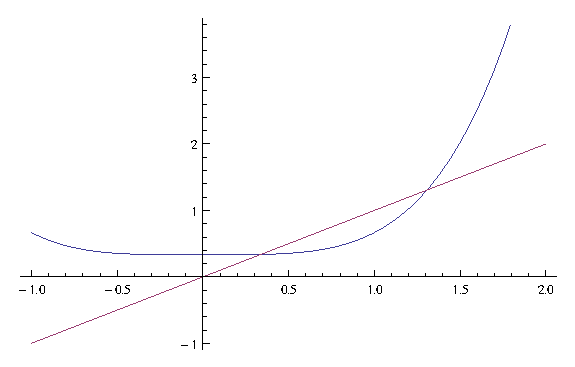
\includegraphics{Analysis/Analysis_sequence.eps}}
\end{figure}

\centertexdraw{
    
    \def\bdot {\fcir f:0 r:0.03 }
    
    \drawdim in

    \arrowheadtype t:F \arrowheadsize l:0.08 w:0.04
    \linewd 0.01 \setgray 0 

    \move (-1 -1) \lvec(2 2)
    \move (-1 0) \clvec (1 0.5)(1.5 1)(2 1.5)
  
    \move (-1 -1) \avec (-1 0 ) \avec(0 0) \avec(0 0.3) \avec(0.3 0.3) \avec(0.3 0.4)
    \move (2 2) \avec (2 1.5) \avec(1.5 1.5) \avec(1.5 1.05) \avec(1.05 1.05) \avec(1.05 0.75) \avec(0.75 0.75) \avec(0.75 0.6)\avec(0.6 0.6)
    
    \move (0.46 0.46) \bdot   
    \htext (-1.1 -1){0}
    \htext (0.4 0.2){$r_1$}

    \move (2 -1) \lvec(5 2)
    \move (2.2 -1) \clvec (3.2 0.5)(3.4 1)(3.7 2)

    \move (2.57 -0.43) \bdot   
    \move (3 0) \avec (3 0.3) \avec (3.3 0.3) \avec (3.3 0.85) \avec (3.85 0.85) \avec (3.85 2) 
    \htext (2.8 -0.5){$r_2$}
 
\move (0 -1.2)
}

Let the two roots of $f(x) = (x^4+1)/3 - x$ be $r_1$ and $r_2$ ($r_1 < r_2$). Because $f(0)>0$, $f(1) <0$ and $f(2) >0$, we have $r_1 \in (0,1)$ and $r_2\in (1,2)$.

Graphical analysis tells us that sequences starting with $a_1 =0,1$ converge to $r_1$ and $a_1 = 2$ diverges to infinity.

$a_1 = 0$. If $a_n \in (0,r_1)$, $f(a_n) = (a_n^4+1)/3 - a_n = a_{n+1} -a_n >0\ \ra \ a_{n+1} > a_n$. But
\be
a_{n+1} = (a_n^4+1)/3 < (r_1^4+1)/3 = r_1   
\ee

Thus, $a_n$ is increasing and bounded above so it is converging.

$a_1 = 1$. If $a_n \in (r_1,r_2)$, $f(a_n) = (a_n^4+1)/3 - a_n = a_{n+1} -a_n < 0\ \ra \ a_{n+1} < a_n$. But
\be
a_{n+1} = (a_n^4+1)/3 > (r_1^4+1)/3 = r_1   
\ee

Thus, $a_n$ is decreasing and bounded above so it is converging.

$a_1 = 2$. If $a_n \in (r_2,\infty)$, $f(a_n) = (a_n^4+1)/3 - a_n = a_{n+1} -a_n >0\ \ra \ a_{n+1} > a_n$. Thus, $a_n$ is increasing and unbounded above so it is diverging.
\end{solution}

%------------------------------------------------------------------------------------------------------------------

\begin{problem}
Let $a_1>b_1>0$ and let $a_{n+1} = (a_n + b_n)/2$, $b_{n+1} = 2a_nb_n/(a_n+b_n)$ for $n\geq 1$. Show that $a_n>a_{n+1}>b_{n+1}>b_n$ and deduce the two sequences converge to a common limit. What limit?
\end{problem}

\begin{solution}[\bf Solution.]
Since $a_1>b_1>0$,
\be
\left\{\ba{l}
2a_1 > a_1 + b_1 \ \ra \ a_1 > \frac{a_1 + b_1}2 = a_2\\
\frac 1{a_1} < \frac 1{b_1} \ \ra \  \frac 1{a_1} + \frac 1{b_1}  < \frac 2{b_1} \ \ra \ b_1 < \frac 2{\frac 1{a_1} + \frac 1{b_1}} = b_2\\
a_2 - b_2 = \frac{a_1 + b_1}2 - \frac {2a_1b_1}{a_1 + b_1} = \frac {(a_1 - b_1)^2}{2(a_1+b_1)} >0
\ea\right. \ \ra \ a_1 > a_2 > b_2 > b_1.
\ee

By induction, we have $a_n>a_{n+1}>b_{n+1}>b_n$. Since $a_n$ is a decreasing sequence, and bounded below (by 0), thus $a_n$ converges to $a$. Similarly, $b_n$ is an increasing sequence and bounded above (by $a_1$). Thus,
\be
\left\{\ba{l}
a = \frac {a+b}2 \\
b = \frac {2ab}{a+b}
\ea\right. \ \ra \ a = b.
\ee
which means that $a_n$ and $b_n$ converge to a common limit $c$. We know that
\be
a_{n+1}b_{n+1} = (a_n + b_n)/2 \times 2a_nb_n/(a_n+b_n) = a_n b_n \ \ra \ c^2 = a_1 b_1 \ \ra \ c = \sqrt{a_1b_1}.
\ee
\end{solution}
